\documentclass[
	12pt, 
	a4paper, 
	openright, 
	twoside
]{abntex2}                                                                          % modelo abntex2(memoir). Fonte 12, papel A4, twoside(ambos lados) e openright(anverso) para elementos pré textuais e novos chapters
% \usepackage{helvet}                                                                 % pacote helvet/arial
% \renewcommand{\familydefault}{\sfdefault}                                           % configura fonte como serif (Arial)
\usepackage[T1]{fontenc}                                                            % fonte
\usepackage[utf8]{inputenc}                                                         % codificação do arquivo tex, caracteres utf8
\usepackage[brazil]{babel}                                                          % hifenização
% \usepackage{sectsty}                                                                % formatação de seções
% \sectionfont{\clearpage}                                                            % nova página para cada seção 
% \usepackage[a4paper,top=3cm,left=3cm,right=2cm,bottom=2cm]{geometry}                % bordas
\PassOptionsToPackage{hyphens}{url}\usepackage{hyperref}                            % formatação de url's e hyperlink neles
% \usepackage[alf, abnt-emphasize=bf]{abntex2cite}                                    % citações estilo ABNT, opção [alf] para citação (autor, data) e [num,overcite] para citação estilo [1]. abnt-emphasize=bf para deixar títulos em negrito https://linorg.usp.br/CTAN/macros/latex/contrib/abntex2/doc/abntex2cite.pdf

\usepackage[alf]{abntex2cite}                                              % citações estilo ABNT, opção [alf] para citação (autor, data) e [num,overcite] para citação estilo [1]. https://linorg.usp.br/CTAN/macros/latex/contrib/abntex2/doc/abntex2cite.pdf
% \citebrackets[]																		% estilo de colchetes para as fontes
% \usepackage[nottoc]{tocbibind}                                                      % opções do sumário, bibliografia no sumário, tirar autorreferência ao sumário 
\usepackage{graphicx}                                                               % imagens e gráficos graphviz
\usepackage{tikz}                                                                   % imagens tikz, usado com dot2tex
\usepackage{amsmath}                                                                % equações
\usepackage{mathtools}                                                              % mais símbolos matemáticos
\usepackage{amssymb}                                                                % símbolos, como flechas e outros
\usepackage{mathrsfs}                                                               % símbolos extras com comando \mathscr, ex: símbolos para transformadas F, Z e L
\usepackage{siunitx}                                                                % unidades SI
\usepackage{indentfirst}                                                            % identar primeira linha depois do comando \section ou \subsection
\usepackage{xcolor}                                                                 % definição de cores, usado na listagem de código
% \renewcommand{\arraystretch}{1.7}                                                   % separação vertical entre células em tabelas
\usepackage{pdfpages}                                                               % inclusão de pdf's

\usepackage{luacode}                                                                % macros para melhor execução de código lua, \luaexec e \begin{luacode} ... \end{luacode}. https://linorg.usp.br/CTAN/macros/luatex/latex/luacode/luacode.pdf
\usepackage{luapackageloader}                                                       % pra máquina lua procurar pacotes nos paths
\directlua{package.path = "./lua/?.lua;" .. package.path }             % anexa o meu path do lua rocks pra pacotes no package.path, mudar se necessário

% comandos para usar no tabular de forma a dar tamanho para as colunas, util para dar espaço extra ou realizar quebra de texto dentro das células. Ex: \begin{tabular}{|cC{2cm}L{4cm}r|}
% left fixed width:
\newcolumntype{L}[1]{>{\raggedright\arraybackslash}p{#1}}
% center fixed width:
\newcolumntype{C}[1]{>{\centering\arraybackslash}p{#1}}
% flush right fixed width:
\newcolumntype{R}[1]{>{\raggedleft\arraybackslash}p{#1}}

% Listagem de código fonte
\usepackage{listings}

\makeatletter
\lst@Key{source}{}{\def\lst@source{#1}} % adicionar opção de fonte
\lst@Key{sourcePrefix}{}{\def\lst@sourcePrefix{#1}} % adicionar opção de prefixo da fonte. Ex: 'Fonte: '

\let\orig@lst@MakeCaption=\lst@MakeCaption % redefinir comando de caption para códigos
\def\lst@MakeCaption#1{%
    \orig@lst@MakeCaption#1%
    \ifx b#1%
        \ifx\lst@source\@empty\else
            \noindent
            \vskip\belowcaptionskip
            \expandafter\lst@makesourcebox\expandafter{\lst@sourcePrefix{} \lst@source{}}%
        \fi
    \fi
}

\def\lst@makesourcebox#1{ % caixa para receber a legenda inferior da fonte
    \makebox[\linewidth][c]{
        \fontfamily{\familydefault}\selectfont
        \footnotesize #1
    }%
}
\makeatother

% estilo da listagem de código
\definecolor{background_color}{HTML}{f8f8fd}
\definecolor{comment_color}{HTML}{6AAF19}
\definecolor{keyword_color}{HTML}{F92672}
\definecolor{ndkeyword_color}{HTML}{00FF00}
\definecolor{string_color}{HTML}{F25A00}
\definecolor{identifier_color}{HTML}{000000}
\definecolor{line_number_color}{HTML}{000000}
\lstdefinestyle{mystyle}{
    backgroundcolor=\color{background_color},   
    commentstyle=\color{comment_color},
    keywordstyle=\color{keyword_color},
    ndkeywordstyle=\color{ndkeyword_color},
    numberstyle=\tiny\color{line_number_color},
    stringstyle=\color{string_color},
    identifierstyle=\color{identifier_color},
    basicstyle=\ttfamily\footnotesize,
    breakatwhitespace=false,         
    breaklines=true,                 
    keepspaces=true,                 
    numbers=left,                    
    numbersep=5pt,                  
    showspaces=false,                
    showstringspaces=false,
    showtabs=false,                  
    tabsize=2,
    captionpos=t,
    aboveskip=15pt,
    belowskip=15pt,
    belowcaptionskip=1ex,
    xleftmargin=1em,
    numbersep=0.5em,
    numberbychapter=false
}
\renewcommand\lstlistingname{Código}
\renewcommand\lstlistlistingname{Códigos}
\lstset{style=mystyle}                                                              % definir estilo de código

% estilo memoir de list, para fazer uma lista de listings
% https://tex.stackexchange.com/a/27648
\begingroup\makeatletter
\let\newcounter\@gobble\let\setcounter\@gobbletwo
	\globaldefs\@ne \let\c@loldepth\@ne
	\newlistof{listings}{lol}{\lstlistlistingname}
	\newlistentry{lstlisting}{lol}{0}
\endgroup
\renewcommand{\cftlstlistingname}{Código\space}
\renewcommand*{\cftlstlistingaftersnum}{\hfill\textendash\hfill}
\newcommand{\listoflistings}{\begin{KeepFromToc}\lstlistoflistings{}\end{KeepFromToc}}

\def\UrlLeft{}                                                                      % tira o sinal < na frente das URLs
\def\UrlRight{}                                                                     % tira o sinal > depois das URLs

\renewcommand{\legend}[1]{                                                          % definir prefixo para comando de legenda de fonte que fica em baixo de figuras e tabelas
    \par
    \centering
    \fontfamily{\familydefault}\selectfont 
    \footnotesize Fonte: #1
}	
\setFloatSpacing{1}																	% espaçamento entre linhas em elementos float(imagens, tabelas e outros) para a legenda e fonte 

\setlength{\cftbeforefigureskip}{0.75ex}                                             % espaçamento de 1.5 na lista de figuras
\setlength{\cftbeforetableskip}{0.75ex}                                              % espaçamento de 1.5 na lista de tabelas

% chapter font config
\renewcommand{\ABNTEXchapterfont}{\fontseries{bx}\fontshape{n}\selectfont}          % estilo da fonte, negrito, não itálico, maiúsculo, tamanho 12pt (\normalsize)
\setboolean{ABNTEXupperchapter}{true}          										
\renewcommand{\ABNTEXchapterfontsize}{\normalsize}         							
\setlength{\beforechapskip}{1.5ex}													% espaçamento entre titulo do capitulo e o paragrafo anterior de aproximadamente 1.5
\setlength{\afterchapskip}{1.5ex}													% espaçamento entre titulo do capitulo e o paragrafo seguinte de aproximadamente 1.5
\setlength{\cftbeforechapterskip}{0.75ex}         									% espaçamento de 1.5 no sumário
\renewcommand{\cftchapterfont}{\ABNTEXchapterfont}                  				% definir mesmo estilo de fonte no sumário
\renewcommand{\cftchapterpagefont}{\cftchapterfont}

% part font config
\renewcommand{\ABNTEXpartfont}{\fontseries{bx}\fontshape{n}\selectfont}             % estilo da fonte, negrito, não itálico, maiúsculo, tamanho 12pt (\normalsize)
% \setboolean{ABNTEXupperpart}{false}            										
\renewcommand{\ABNTEXpartfontsize}{\normalsize}            							
% \setlength{\beforepartskip}{1.5ex}													% espaçamento entre titulo da parte e o paragrafo anterior de aproximadamente 1.5
% \setlength{\afterpartskip}{1.5ex}													% espaçamento entre titulo da parte e o paragrafo seguinte de aproximadamente 1.5
% \setlength{\cftbeforepartskip}{1.5ex}            									% espaçamento de 1.5 no sumário
% \renewcommand{\cftpartfont}{\ABNTEXpartfont}                        				% definir mesmo estilo de fonte no sumário
% \renewcommand{\cftpartpagefont}{\cftpartfont}

% section font config
\renewcommand{\ABNTEXsectionfont}{\fontseries{m}\fontshape{n}\selectfont}           % estilo da fonte, não negrito, não itálico, maiúsculo, tamanho 12pt (\normalsize)
\setboolean{ABNTEXuppersection}{true}          										
\renewcommand{\ABNTEXsectionfontsize}{\normalsize}  
\setlength{\beforesecskip}{1.5ex}													% espaçamento entre titulo da seção e o paragrafo anterior de aproximadamente 1.5
\setlength{\aftersecskip}{1.5ex}       												% espaçamento entre titulo da seção e o paragrafo seguinte de aproximadamente 1.5
\setlength{\cftbeforesectionskip}{0.75ex}         									% espaçamento de 1.5 no sumário
\renewcommand{\cftsectionfont}{\ABNTEXsectionfont}                  				% definir mesmo estilo de fonte no sumário
\renewcommand{\cftsectionpagefont}{\cftsectionfont}

% subsection font config
\renewcommand{\ABNTEXsubsectionfont}{\fontseries{b}\fontshape{n}\selectfont}        % estilo da fonte, negrito, não itálico, minúsculo, tamanho 12pt (\normalsize)
\setboolean{ABNTEXuppersubsection}{false}      										
\renewcommand{\ABNTEXsubsectionfontsize}{\normalsize}      
\setlength{\beforesubsecskip}{1.5ex}   												% espaçamento entre titulo da sub seção e o paragrafo anterior de aproximadamente 1.5
\setlength{\aftersubsecskip}{1.5ex}    												% espaçamento entre titulo da sub seção e o paragrafo seguinte de aproximadamente 1.5
\setlength{\cftbeforesubsectionskip}{0.75ex}      									% espaçamento de 1.5 no sumário
\renewcommand{\cftsubsectionfont}{\ABNTEXsubsectionfont}            				% definir mesmo estilo de fonte no sumário
\renewcommand{\cftsubsectionpagefont}{\cftsubsectionfont}

% subsubsection font config
\renewcommand{\ABNTEXsubsubsectionfont}{\fontseries{m}\fontshape{n}\selectfont}    % estilo da fonte, não negrito, itálico, minúsculo, tamanho 12pt (\normalsize)
\setboolean{ABNTEXuppersubsubsection}{false}   										
\renewcommand{\ABNTEXsubsubsectionfontsize}{\normalsize}   
\setlength{\beforesubsubsecskip}{1.5ex}												% espaçamento entre titulo da sub sub seção e o paragrafo anterior de aproximadamente 1.5
\setlength{\aftersubsubsecskip}{1.5ex} 												% espaçamento entre titulo da sub sub seção e o paragrafo seguinte de aproximadamente 1.5
\setlength{\cftbeforesubsubsectionskip}{0.75ex}   									% espaçamento de 1.5 no sumário
\renewcommand{\cftsubsubsectionfont}{\ABNTEXsubsubsectionfont}      				% definir mesmo estilo de fonte no sumário
\renewcommand{\cftsubsubsectionpagefont}{\cftsubsubsectionfont}

% nome de seção em maiúsculo no sumário
% https://tex.stackexchange.com/a/399861
\makeatletter
\let\oldcontentsline\contentsline
\def\contentsline#1#2{%
	\expandafter\ifx\csname l@#1\endcsname\l@section
		\expandafter\@firstoftwo
	\else
		\expandafter\@secondoftwo
	\fi
	{%
		\oldcontentsline{#1}{\MakeTextUppercase{#2}}%
	}{%
		\oldcontentsline{#1}{#2}%
	}%
}
\makeatother

% ajustes para anexo maiúsculo no sumário, no caso de Sumario (TOC) especifico da ABNT-6027-2012 precisa desse debaixo pro anexo ficar minúsculo
% \makeatletter
% \ifthenelse{\boolean{ABNTEXsumario-abnt-6027-2012}}{
% \settocpreprocessor{chapter}{%
%     \let\tempf@rtoc\f@rtoc%
%     \def\f@rtoc{%
%         \texorpdfstring{\MakeTextUppercase{\tempf@rtoc}}{\tempf@rtoc}}%
% }
% \settocpreprocessor{part}{%
%     \let\tempf@rtoc\f@rtoc%
%     \def\f@rtoc{%
%         \texorpdfstring{\MakeTextUppercase{\tempf@rtoc}}{\tempf@rtoc}}%
% }
% \settocpreprocessor{subsection}{%
%     \let\tempf@rtoc\f@rtoc%
%     \def\f@rtoc{%
%         \texorpdfstring{\MakeTextUppercase{\tempf@rtoc}}{\tempf@rtoc}}%
% }
% }{}
% \makeatother

% citação direta
\setlength{\ABNTEXcitacaorecuo}{4cm}

\renewenvironment{citacao}{
\begin{flushright}
\begin{SingleSpace}
\begin{minipage}{\textwidth - \ABNTEXcitacaorecuo + \foremargin}
\ABNTEXfontereduzida
}{      
\hspace{0.05\textwidth}
\end{minipage}
\end{SingleSpace}
\end{flushright}
}

\setlength{\ABNTEXsignwidth}{8.5cm}                                                 % largura da assinatura na folha de aprovação

\OnehalfSpacing                                                                     % espaçamento entre linhas

\counterwithout{equation}{chapter}                                                  % não enumerar equações por capitulo, fazer de forma contínua por todo o documento 

% https://linorg.usp.br/CTAN/macros/latex/contrib/memoir/memman.pdf#page=83
\captionnamefont{\ABNTEXfontereduzida}                                              % tamanho das legendas
\captiontitlefont{\ABNTEXfontereduzida}                                             % tamanho das legendas

% tipo de página, cabeçalho só mostra o número da página
\makepagestyle{simple-folio}
\makeevenhead{simple-folio}{\ABNTEXfontereduzida\thepage}{}{}
\makeoddhead{simple-folio}{}{}{\ABNTEXfontereduzida\thepage}
\directlua{require("lua/tablecsv.lua")}

% open file to be used by subsequent calls
% arg1: filename
\newcommand\openfile[1]{\luaexec{openFile(\luastring{#1},",",true)}}

% get a field value by col row reference
% arg1: col
% arg2: row
\newcommand\getfield[2]{\luaexec{getField(#1,#2)}}

% get a range from the opened file formatted for tex tabular's. Ex: "1 & 2 & 3 \\\hline"
% arg1: first col
% arg2: first row
% arg3: second col
% arg4: second row
\newcommand\tabularfromrange[4]{\luaexec{tabularFromRange(#1,#2,#3,#4)}}
% arg5: line ending. If not provided defaults to "\hline"
% \newcommand\getrange[5]{\luaexec{getRange(#1,#2,#3,#4,\luastring{#5})}}

%%%%%%%%%%%%%%%%%%%%%%%%%%%%%%%%%%%%%%%%%%%%%%%%%%%%%%%%%%%%%%%%%%%%%%%%%%%%%%%%%%%%%%%%%%%%%%%%

\titulo{Desenvolvimento de um método e sistema para compilação e simulação de redes de petri para utilização em  controladores lógicos industriais}              								% titulo do trabalho
\autor{João Peterson Scheffer}                 							% nome do discente
\local{Luzerna}	               								% local/cidade
\def\estado{SC}												% estado, formato duas letras. Ex: SC, PR, SP 
\data{Dezembro de 2022}       								% data da capa
\def\Data{08 de dezembro de 2022}                      		% data da folha de aprovação
\def\instituicaoartigo{do}									% artigo para se referir a instituição. Ex: 'da' Universidade, 'do' Instituto
\def\nomeinstituicao{Instituto Federal Catarinense}		% nome da instituição
\def\curso{Bacharelado em Engenharia de Controle e Automação}							% curso. Ex: Bacharelado em XXX, Licenciatura em XXXX
\def\cursotitulo{Bacharel em Engenharia de Controle e Automação}							% titulo a quem se forma no curso. Ex: Bacharel em XXXX
\def\campus{Campus \imprimirlocal}							% campus. Ex: Campus Luzerna
\instituicao{ 												% instituição, curso e campus
	\nomeinstituicao
	\par
	\curso
	\par
	\textit{\campus}
}

\tipotrabalho{Trabalho de conclusão (Bacharelado)} 			% tipo de trabalho, usado na ficha catalográfica Ex: Trabalho de conclusão (Bacharelado), Tese (Doutorado), Dissertação (Mestrado).
\orientador{Prof. Msc. Tiago Javorani Prati} 								% nome do orientador
% \coorientador{Prof. Msc. NOME} 							% nome do coorientador
\def\primeiroavaliador{Prof. Msc. XXXXXXX}           		% primeiro avaliador
\def\primeiroavaliadorafiliacao{							% instituição do primeiro avaliador
	Instituto Federal Catarinense
}           		
\def\segundoavaliador{Prof. Dr. XXXXXX}              		% segundo avaliador
\def\segundoavaliadorafiliacao{								% instituição do segundo avaliador
	Instituto Federal Catarinense
}           		
\def\PalavrasChave{	                                 		% palavras chave para o resumo
	redes de petri; automação industrial; \textit{software}.
} 
\def\Keywords{												% palavras chave para o resumo em inglês
	petri nets; industrial automation; \textit{software}.
}
\preambulo{													% O preambulo deve conter o tipo do trabalho, o objetivo, o nome da instituição e a área de concentração 
	Trabalho de conclusão apresentado à banca examinadora do curso de \curso, do \nomeinstituicao, \campus, como requisito para a obtenção do título de \cursotitulo, em cumprimento às exigências de sua componente curricular.
}

%%%%%%%%%%%%%%%%%%%%%%%%%%%%%%%%%%%%%%%%%%%%%%%%%%%%%%%%%%%%%%%%%%%%%%%%%%%%%%%%%%%%%%%%%%%%%%%%
\renewcommand{\imprimircapa}{
\begin{capa}
\begin{center}
	\begin{SingleSpace}
	\begin{figure}[!ht]
		\centering
		
\includegraphics[width = 0.25\textwidth]{images/logo.png}
	\end{figure} 

	\imprimirinstituicao
	
	\vspace*{2ex}
	{\ABNTEXchapterfont\imprimirautor}
	
	\vfill
	
	{\ABNTEXchapterfont\imprimirtitulo}
	\end{SingleSpace}
	
	\vfill

	\imprimirlocal \\
	\imprimirdata
\end{center}
\end{capa}
}
\renewcommand{\folhaderostocontent}{
\begin{center}
	
	{\ABNTEXchapterfont\imprimirautor}

	\vfill

	{\ABNTEXchapterfont\imprimirtitulo}
	
	\vfill

	\hspace{.45\textwidth}
	\begin{minipage}{.5\textwidth}
	\begin{SingleSpace}
		\imprimirpreambulo
		Orientador: \imprimirorientador
	\end{SingleSpace}
	\end{minipage}
	
	\vfill
	
	\imprimirlocal \\
	\imprimirdata
\end{center}  
}
\makeindex

\begin{document}
\pretextual
\imprimircapa
\imprimirfolhaderosto

% Isto é um exemplo de Folha de aprovação, elemento obrigatório da NBR
% 14724/2011 (seção 4.2.1.3). Você pode utilizar este modelo até a aprovação
% do trabalho. Após isso, substitua todo o conteúdo deste arquivo por uma
% imagem da página assinada pela banca com o comando abaixo:

% \includepdf{folhadeaprovacao_final.pdf}

\begin{folhadeaprovacao}
\DoubleSpacing
\begin{center}

	{\ABNTEXchapterfont\imprimirautor}

	\vfill

	{\ABNTEXchapterfont\imprimirtitulo}

	\vspace*{1cm}

	\hspace{.45\textwidth}
	\begin{minipage}{.5\textwidth}
	\begin{SingleSpace}
		\imprimirpreambulo
	\end{SingleSpace}
	\end{minipage}

	\vspace*{1.5cm}
	
	\imprimirlocal ~(\estado), \Data :
	
	\assinatura{\textbf{\imprimirorientador} \\ \nomeinstituicao}
	
	\vspace*{1.5cm}
	\textbf{BANCA EXAMINADORA}

	\assinatura{\textbf{\primeiroavaliador}\\ \primeiroavaliadorafiliacao}
	\assinatura{\textbf{\segundoavaliador}\\ \segundoavaliadorafiliacao}	
\end{center}
\end{folhadeaprovacao}
% \begin{dedicatoria}
\vspace*{\fill}
Exemplo: Este trabalho é dedicado aos meus colegas de classe, aos meus queridos pais e professores
\end{dedicatoria}

\begin{agradecimentos}
Deixo meus agradecimentos primeiramente aos meus pais e familia, que me incentivaram, apoiaram e me custodiaram durante minha formação, espero que estejam orgulhosos de mim. Agradecimento aos meus amigos, colegas e corpo do IFC Luzerna, que me deram durante minha formação um ambiente não só de educação e desenvolvimento intelectual mas também de amadurecimento, onde pude me desenvolver como pesoa e ser quem sou hoje, resguardo assim um carinho imenso por esta época da minha vida e das pessoas que me acompanharam.

Agradeço ao professor Thiago Javorani Prati, meu orientador, que em aula me apresentou aos conceitos principais tratados neste trabalho, quais tomei gosto e agora culmina-se em uma nova obra.

Agradeço também aos professores Ricardo Kerschbaumer, Marcelo Cendron e Ricardo Antonello, cada qual de maneiras diferentes inspiraram minha paixão pelo mundo da programação, que é meu foco atual, seja na minha profissão ou mesmo neste trabalho.
\end{agradecimentos}
% \begin{epigrafe}
\vspace*{\fill}
\hspace{.45\textwidth}
\begin{minipage}{.5\textwidth}
\itshape
	
	Texto da Epígrafe. Citação relativa ao tema do trabalho. É opcional. A epígrafe pode também aparecer na abertura de cada seção. Deve ser elaborada de acordo com a NBR 10520. \\

	\begin{flushright}		
	(SOBRENOME do autor da epígrafe, ano) 
	\end{flushright}
\end{minipage}
\end{epigrafe}
\setlength{\absparsep}{18pt} % ajusta o espaçamento dos parágrafos do resumo
\begin{resumo}

O presente trabalho propõe o desenvolvimento de um método e sistema para a simulação/execução de redes de petri e compilação para código de lista de instrução para controladores lógicos programáveis. As redes de petri são uma poderosa ferramenta para modelar e automatizar sistemas industriais, permitindo representar o comportamento de diferentes processos e eventos de forma eficiente e complementar aos métodos de programação tradicionais. No entanto, a utilização dessas redes em \textit{software}, com ênfase em controladores lógicos programáveis, é geralmente feita de forma manual, sendo o \textit{design} da rede realizada em uma etapa e a posteriormente convertida para \textit{software}. Portanto, há espaço e demanda para criação de ferramentas e métodos para utilização dessa tecnologia de forma mais simples e integrada.

A base para implementação dessa tecnologia é um sistema capaz de representar e executar essas redes. Portanto, é proposto o desenvolvimento de uma biblioteca em linguagem C que apresenta as funções de representação, checagem, simulação/execução e armazenamento de redes de petri, podendo ser usada em computadores \textit{desktop} e sistemas embarcados. 

Para o uso em controladores lógicos programáveis, propõem-se um algoritmo de compilação que traduz as especificações de uma rede de petri na biblioteca C para um conjunto de instruções adequadas para o controlador lógico industrial, nesse trabalho em específico, o controlador WEG TPW04. A compilação permite que a rede seja executada diretamente pelo controlador, garantindo a funcionalidade desejada e uma integração mais trivial com o ambiente industrial.

Espera-se que o método e sistema desenvolvidos neste trabalho contribuam significativamente para o avanço da aplicação prática de redes de petri em meio industrial, provendo uma ferramenta complementar a outros métodos para os desenvolvedores de aplicações industriais e \textit{software} em geral.
	
\textbf{Palavras-chave}: Redes de petri; Automação industrial; PLC; Linguagem C.
\end{resumo}

\begin{resumo}[Abstract]
\begin{otherlanguage*}{english}
The following work presents the development of a method and system for simulating/executing petri nets and compilation to instruction list code for usage on programmable logic controllers. Petri nets are a powerful tool for modeling and automating industrial systems, enabling the representation of the behavior for different processes and events in an efficient manner and complimentary to tradicional programming methods. But, the use of these nets in software, with emphasis on programmable logic controllers, is generally made by hand, in which the petri net is designed first and then converted to software. Therefore,  there is space and demand for the conception of tools and methods for the utilization of this technology in a more simple and integrated manner. 

The base for this implementation is a system capable of representing and executing these nets. Therefore,  it is proposed the development of a C library that features the representation, checking, execution and storage of petri nets, capable of being used in desktop and embedded systems applications. 

For usage with programmable logic controllers, it is proposed an compilation algorithm that translates the specifications of a given petri net in the C library to a set of instructions for the programmable logic controller, in specific for this implementation, the WEG TPW04 controller. The compilation enables the controller to execute the petri net directly, granting the desired functionality and a more trivial integration with the industrial environment.

It is hoped that the method and system developed in this work contributes significantly for the advance of the practical use of petri nets in industrial environments, providing a tool that is complementary to other programming methods for the development of industrial applications as well as in general software.

\textbf{Keywords}: Petri nets; Industrial automation; PLC; C language.
\end{otherlanguage*}
\end{resumo}
\pdfbookmark[0]{\listfigurename}{lof}						% lista de ilustrações
\listoffigures*
\cleardoublepage

\pdfbookmark[0]{\listtablename}{lot} 						% lista de tabelas
\listoftables*
\cleardoublepage

\pdfbookmark[0]{\listtablename}{lol} 						% lista de códigos
\listoflistings
\cleardoublepage

\begin{siglas}												% lista de abreviaturas e siglas
    \item[PLC]               \textit{Programmable logic controller}
    \item[CLP]               Controlador lógico programável
    \item[WYSIWYG]           \textit{What you see is what you get}
    \item[Vscode]            \textit{Visual studio code}
\end{siglas}

% \begin{simbolos}											% lista de símbolos
% 	\item[$\xi $]           Coeficiente de amortecimento
% \end{simbolos}

\pdfbookmark[0]{\contentsname}{toc}  						% sumario
\tableofcontents*
\cleardoublepage
%%%%%%%%%%%%%%%%%%%%%%%%%%%%%%%%%%%%%%%%%%%%%%%%%%%%%%%%%%%%%%%%%%%%%%%%%%%%%%%%%%%%%%%%%%%%%%%%
\textual
\pagestyle{simple-folio}                                                            % sem nome do capitulo no cabeçalho
\chapter{Introdução}

Quando se trata de sistemas dinâmicos como um todo há sempre um interesse de criar, entender, prever e controlar estes sistemas, e no âmbito de sistemas discretos orientados a eventos \footnote{Sistemas que trabalham com valores discretos como ligado e desligado por exemplo e possuem mudança de estado conforme eventos também discretos.}, como alguns sistemas industriais de automação de interesse neste trabalho, há várias metodologias, práticas, tecnologias e linguagens de programação capazes de trabalhar estes sistemas de forma a alcançar resultados esperados, cada qual possuí vantagens e desvantagens.

No âmbito industrial, para realizar o controle e automação de processos, comumente é utilizado controladores lógicos programáveis, PLC's, e estes podem ser programados para realizar as funções desejadas e para isso empregam a utilização de linguagens de programação como: 

\begin{itemize}
	\item \textit{Ladder}, que representa um processo de forma visual inspirada em lógica de contatos \footnote{Uma forma simples de programação baseada na representação visual de lógica de contato, como vista em diagramas com relés e contatoras.}.
	\item Lista de instrução, que é uma linguagem escrita, não visual, e que representa um fluxo de operações com base em comandos de texto.
	\item Grafcet, uma linguagem visual que representa um processo em forma de fluxo com base em passos de um nó para outro nó do processo, onde cada nó é uma instrução de ação e cada passo é dado conforme uma transição atrelada a um evento. 
\end{itemize}

Ainda há outras tecnologias que possuem outras formas abstratas e abordagens diferentes, sendo a linguagem \textit{Ladder} um exemplo de aproveitamento de conhecimento e simplicidade, porém há casos onde certas ferramentas não apresentam melhor desempenho e eficiência dado certos tipos de especificações, em especial no caso do \textit{Ladder}, onde controle de estado \footnote{Armazenamento e lógica do estado/situação atual de um processo} e paralelismo \footnote{Capacidade de unir dois fluxos de trabalho com razões de trabalho diferentes em um ponto definido.} são conceitos difíceis de serem implementados. 

Para resolver algum destes problemas, condições e situações como as mencionadas, emprega se o uso de linguagens de modelagem lógica capazes de definir um sistema desejado, representa lo como um sistema discreto orientado a eventos, onde podem se empregar abstrações lógicas adequadas a situação ou ainda prover ferramentas para realizar análise como alcançabilidade, significando se existem casos passíveis de serem realizados apesar da intenção contrária do projeto, se o sistema é reinicializável, significando a possibilidade do sistema de retornar a um estado inicial sempre, dentre outras análises complexas.

Neste contexto há varias linguagens de modelagens lógicas, como autômatos, máquinas de \textit{Moore}, dentre outras linguagens lógicas, que podem ser usadas para abstrair alguns conceitos como os citados anteriormente e nesse contexto apresenta se então a rede de Petri \cite{scholarpedia2011}, que é capaz de reproduzir conceitos abstratos como paralelismo, sincronia, mutualidade exclusiva, etc., de forma simples bem como vários outros conceitos comuns de lógica e aritmética e conceitos ainda exclusivos, intrínsecos a si própria. 

As redes de Petri são assim um instrumento de maior formalidade e podem representar conceitos abstratos, fazendo da mesma uma ótima ferramenta para automação e controle de sistemas a eventos discretos, e que cada vez mais vem sendo estudada em meio acadêmico quanto a sua utilização como mecanismo de modelagem de processos, modelagem de sistemas criticos \cite{1702225} e \cite{ghezzi1991unified}, e prevenção de \textit{deadlocks} \footnote{Singularidade em processos onde o sistema entra em um ponto de parada de forma imprevista e não possuí forma de autocorreção, permanece ou parado em falha ou em repetição contínua de uma única instrução.} \cite{kaid2015applications}.

Visto o um grau de interesse acadêmico, aplicações em situações bem definidas, significando se tratar de uma ferramenta adequada, e ainda a utilidade industrial, dado sua ótima representação de processos e liberdade de abstração, pode se dizer que há interesse prático em redes de petri, porém o emprego real deste tipo de tecnologia é mínimo, existem metodologias \cite{6621049} que por exemplo, propõem a funcionalidade de interpretação de redes de petri de alto nível para código \textit{Ladder} capaz de ser então usado em PLC's para uso industrial, função implementada em projetos como \textit{PetriLab} \cite{de2015petrilab}, porém não trazem integração real, uma boa experiência de programação ou mesmo boas práticas de design de \textit{software}, características que são valorizadas e por vezes indispensáveis para o processo de desenvolvimento, integração, teste, manutenção e melhoria contínua de sistemas e controle de sistemas em meio industrial, em outras palavras, há necessidade de ferramentaria adequada e atrativa as empresas e desenvolvedores destes sistemas industriais bem como difusão da utilização de redes de petri como ferramenta de uso geral e específico.

\section{Justificativa}

Sendo apresentado o estado atual de disseminação de utilização de redes de petri, tanto geral como industrial, justifica se a criação de ferramentaria necessária ao desenvolvimento de aplicações. Aplicações tais que implementam necessariamente formas visuais de representação e edição, bem como simulação e observação do funcionamento destas redes e ainda a funcionalidade de transformar estas redes em programas prontos para utilização em meio industrial.

A capacidade de transformar tais redes em programas industriais, compreende se como o processo de trans compilação, onde a rede de petri é traduzida através de um algoritmo proposto para o resultado de saída, sendo esta saída código puro, arquivos digitais ou programas prontos pra utilização com PLC's industriais.

\section{Objetivos}

\subsection{Objetivo geral}

Desenvolvimento de um ambiente de edição, simulação e compilação de rede de petri voltadas para utilização em meio industrial, PLC's.

\subsection{Objetivos específicos}

\begin{itemize}
	\item Desenvolvimento de uma biblioteca implementada em linguagem C, contendo uma estrutura de dados que represente a rede de petri em memória e que implemente a dinâmica de funcionamento, a simulação.
	
	\item Desenvolvimento de algoritmos de trans compilação de redes de petri para o seguinte alvo:
	\begin{itemize}
		\item Lista de instrução, em formato de texto.
	\end{itemize}

	\item Desenvolvimento de uma aplicação gráfica para edição e simulação de redes de petri utilizando o \textit{framework} Flutter com linguagem de programação Dart.

	\item Desenvolvimento de uma biblioteca em Dart que porta as funções da biblioteca em linguagem C para utilização dentro do \textit{framework} Flutter.
\end{itemize}
\chapter{Metodologia}

Este trabalho se trata de um processo de desenvolvimento pelo do autor de maneira autônoma, dado que os tópicos de programação e alguns detalhes de implementação são por natureza de livre implementação, tornando este trabalho por grande parte um trabalho exploratório. 

\section{A base do projeto}

Para implementação do sistema proposto, é necessário entender que deseja-se que os resultados do sistema, as redes de petri, sejam acessíveis em várias plataformas, visando-se generalização. Entende-se assim que deve-se haver um motor capaz de executar estas redes e seu funcionamento em suas respectivas plataformas. Em computadores de uso geral, e em sistemas embarcados torna-se atrativo uma implementação na forma de uma biblioteca em linguagem C, pois a maioria dos sistemas embarcados funcionam com \textit{toolchains}\footnote{Conjunto de ferramentas que possibilitam a programação e manuseio de programas para uma plataforma e/ou arquitetura de computador específica.} em C, e também pois abre-se as portas para que outros ambientes e linguagens de programação utilizem esta biblioteca. Isto é possível pelo fato de C ser de baixo nível e seguir padrões estabelecidos de arquivos e execução de código no geral, tornando possível que linguagens de mais alto nível possam fazer \textit{bindings}\footnote{Sistema onde se mapeia de forma diretas funções, variáveis e definições de código entre sistemas/ambientes de programação diferentes, possibilitando interoperabilidade entre elas} para com a biblioteca. 

Mais ainda, outro motor importante é a capacidade de executar tais redes em plataformas distintas, onde a portabilidade da biblioteca em C torna-se difícil, como os PLC's comentados anteriormente, onde a lista de instrução é mais comum do que a linguagem C. A lista de instrução, tanto pela difusão quanto pelo baixo nível de abstração, um candidato preferido para alvo de compilação, assim a rede pode ser editada, simulada e testada em um computador de uso geral, por exemplo, e então compilada para lista de instrução, que deve ser gerada de forma a garantir funcionalidade igual a da biblioteca em C.

O baixo nível de abstração da lista de instrução ainda possibilita que esta seja usada como fonte para compilação posterior por ferramentas de terceiros para suas plataformas alvo, abrindo mais funcionalidade para esse tipo de sistema de trabalho. Por exemplo, lista de instrução é comumente compilada para \textit{Ladder} de forma intercambiável, ou seja, é um processo bidirecional, comportamento desejado por desenvolvedores, dado que \textit{Ladder} é uma linguagem visual simples e de mais fácil desenvolvimento do que a lista de instrução pura.

Para implementação da representação das redes, da dinâmica e da compilação será utilizada a linguagem C bem como um sistema de compilação para a biblioteca usando ferramentas básicas no padrão POSIX\nocite{posix}, em especial do projeto GNU \cite{gnu} sendo elas o compilador \textit{gcc}, e para \textit{build}\footnote{Processo organizado de construção de um programa ou biblioteca a partir de diferentes arquivos fonte, que são compilados e ligados conforme a necessidade do projeto.} o \textit{Make}.

% \section{Parte visual}

% No que se refere ao aspecto visual, temos o desenvolvimento de uma aplicação de edição para qual foi tomada inspiração do trabalho anterior Petrilab \cite{de2015petrilab} bem como o editor de texto Visual Studio Code \cite{vscode}. Para o desenvolvimento desta aplicação devemos pensar que a mesma será utilizada em computadores desktop, será escolhido assim um framework visando funcionamento em diversos sistemas operacionais, facilidade e tendencias modernas, como o framework Flutter\cite{flutter}. 

% O mesmo possui uma metodologia moderna de desenvolvimento de aplicações visuais bem como a capacidade de ter como linguagem de programação o Dart, qual possui interoperabilidade com C, podendo assim a aplicação visual utilizar a biblioteca em C para simulação a rede de petri criada.

\section{Rede de petri}

Quanto a definição do tipo de rede de petri adotada neste trabalho, serão adotadas redes de petri com extensões específicas e utilidade geral de e industrial, garantindo maior flexibilidade no design. A definição destas extensões e os detalhes de implementação serão discutidos e embasados conforme trabalhos anteriores bem como a experiência prática do autor.

\section{Compilador de lista de instrução}

Lista de instrução é um tipo de programação relativamente difundida e portanto bem generalizada, mas ainda assim há diferenças entre fabricantes. Em vista disto, a implementação do compilador de rede de petri para lista de instrução proposta neste trabalho irá utilizar uma implementação específica, sendo esta a referência da fabricante WEG para o PLC TPW04 \cite{wegtpw04}, sendo este um modelo amplamente utilizado em meio industrial e também de fácil acesso em educacional e acadêmico. Futuros trabalhos podem partir da mesma referência para implementação de compiladores para mais arquiteturas de PLC's, dada que as diferenças de implementação são pequenas entre tipos de plataformas e fabricantes diferentes devido a norma IEC 61161-3 \cite{IEC611313}.  

\section{Publicação}

Todo o trabalho desenvolvido nesta obra será versionado e disponibilizado no repositório "pnet" \cite{github-pnet} via Github \cite{github}, sob a licença domínio público MIT \cite{mit-license}.

% Todo o trabalho desenvolvido nesta obra será versionado e disponibilizado como repositórios distintos via Github \cite{github}, todos sob a licença domínio público MIT \cite{mit-license}, sendo estes repositórios o da biblioteca C \cite{github-pnet}, da aplicação visual Flutter \cite{github-petricad} e do plugin Flutter que irá encapsular a funcionalidade da biblioteca em C via bindings utilizando as capacidades da linguagem Dart \cite{github-pnet-dart}.
\chapter{Fundamentação teórica}

Nesta introdução teórica, será abordado o funcionamento básico das redes de petri e alguns dos principais tipos existentes. É importante compreender esses conceitos fundamentais antes de prosseguir para a implementação de \textit{software}, pois definirá a ideia de funcionamento e implementação, onde poderá se observar a utilidade das redes, possíveis abstrações e comportamentos desejados, como os de interesse abordados na seção de introdução. Também conceitos relacionados a implementação de \textit{software} e outros conceitos adjacentes necessários ao entendimento do desenvolvimento das partes integrantes do trabalho.

\section{Redes de petri}

As redes de petri são uma poderosa ferramenta para a modelagem e análise de sistemas concorrentes e paralelos. Introduzidas por Carl Adam Petri em 1962 \cite{carlpetri}, as redes de petri fornecem uma representação gráfica e formal para descrever a dinâmica de sistemas complexos, permitindo a análise de propriedades importantes, como comportamento temporal, concorrência e paralelismo.

Uma rede de petri é composta por lugares, transições, fichas e arcos. Cada componente tem um papel fundamental na representação e modelagem do sistema.

\begin{itemize}
	\item Lugares: Os lugares representam estados ou condições do sistema. Eles são representados por círculos em um diagrama de rede de petri. Os lugares podem conter fichas, que são unidades discretas que refletem o estado atual do sistema.
	
	\item Transições: As transições representam eventos ou ações que podem ocorrer no sistema. Elas são representadas por retângulos em um diagrama de rede de petri. Para que uma transição seja disparada, é necessário que todos os lugares de entrada estejam marcados com pelo menos uma ficha.
	
	\item Fichas: As fichas são unidades discretas que se movem entre os lugares em resposta à ocorrência das transições. Elas refletem o estado atual do sistema e representam o fluxo de controle. Quando uma transição é disparada, ela consome as fichas dos lugares de entrada e produz novas fichas nos lugares de saída.
	
	\item Arcos: Os arcos conectam os lugares às transições e vice-versa. Eles indicam as relações de dependência entre os elementos do sistema. Existem dois tipos de arcos: arcos de entrada, que conectam lugares a transições, indicando que os lugares são precondições para a ocorrência da transição, e arcos de saída, que conectam transições a lugares, indicando que as transições produzem fichas nos lugares de saída. Estes arcos podem ainda conter pesos, desta forma, um arco de entrada pode retirar mais de uma ficha de um lugar, ou um arco de saída pode inserir várias fichas em outro lugar.
\end{itemize}

\begin{figure}[ht]
	\centering
	\caption{Rede de petri com dois lugares e uma transição}
	%\incsvg{path/}{path/file}
	\incsvg{images}{images/samplepetri}\\
	\label{fig:samplepetri}
\end{figure}

\pagebreak

O funcionamento de uma rede de petri ocorre através de um processo chamado de disparo. Quando todas as condições de precondições de uma transição são satisfeitas, a transição é disparada, consumindo as fichas dos lugares de entrada e produzindo fichas nos lugares de saída correspondentes. Esse processo de disparo ocorre de forma determinística, onde as transições só podem ser disparadas quando todas as condições são atendidas.

Em mais detalhes, as fichas só se movem de um lugar ao outro caso uma transição aconteça, e ela só irá acontecer se o arco for atendido, por exemplo, o arco de peso de saída só irá permitir que a transição ocorra caso a quantidade de fichas no lugar de origem for maior ou igual ao peso, efetivamente colocando uma condição de disparo. Quando todas as condições atreladas a uma transição são atendidas, tal transição diz se sensibilizada. 

\subsection{Tipos de Redes de petri}

Existem vários tipos de redes de petri, cada um com suas características e aplicabilidades específicas. Alguns dos principais tipos são:

\begin{itemize}
	\item Redes de petri coloridas \cite{coloredpetrinets}: Nesse tipo de rede, além das fichas, são utilizadas cores para representar diferentes propriedades ou atributos dos elementos do sistema. Isso permite uma modelagem mais expressiva, onde as cores das fichas podem influenciar o comportamento das transições.
	
	\item Redes de petri temporizadas \cite{petrinetmodeling}: Nesse tipo de rede, são adicionadas informações de tempo às transições e arcos. Essas informações podem incluir atrasos, tempo de execução ou intervalos de tempo específicos para a ocorrência de eventos. Isso possibilita a análise de propriedades temporais e a simulação de sistemas baseados em tempo.
	
	\item Redes de petri estocásticas \cite{stochasticpetrinets}: Nas redes de petri estocásticas, são incorporadas probabilidades às transições e arcos, permitindo a modelagem de sistemas com comportamento probabilístico. Essas redes são úteis para a análise de sistemas em que a ocorrência de eventos é incerta ou aleatória.
	
	\item Redes de petri priorizadas \cite{petrinetmodeling}: Redes onde as transições tem a propriedade de serem priorizadas para disparo em relação ao outras, úteis em caso de disparo simultâneo de uma ou mais transições.

	\item Redes de petri de alto nível \cite{highlevelpetrinets}: As redes de petri de alto nível são uma extensão das redes de petri tradicionais, que permitem uma representação mais abstrata e simplificada dos sistemas. Elas são úteis para modelar sistemas complexos e lidar com a explosão combinatória que pode ocorrer em redes de petri tradicionais. Abstrações como lugares compartilhados, macro transições e hierarquia de sub-redes são utilizadas para simplificar a representação e análise desses sistemas.
\end{itemize}

Esses são apenas alguns dos principais tipos de redes de petri, e cada um deles oferece recursos e abordagens específicas para a modelagem e análise de sistemas. O uso correto e adequado desses tipos de redes de petri depende das características do sistema a ser modelado e das propriedades que se deseja analisar. 

\subsection{Delimitação de uma rede para uso industrial}

As redes de petri são particularmente interessantes, pois apresentam um bom grau de flexibilidade e capacidade de abstração, podendo comportar lógicas completas, simples e robustas, então é de interesse delimitar o tipo de rede que deverá ser trabalhada de forma que possamos ter as funcionalidades e características para modelagem de sistemas, como preferência para sistemas de automação industrial. 

O \textit{software} Petrilab \cite{de2015petrilab} abre o caminho com uma delimitação interessante e prática para uso industrial, onde se propõe a utilização de métodos de entrada e saída para rede de petri, condições lógicas que permitem o acionamento de transições e os tipos de arcos desejados, sendo eles os de peso e arcos negados. Baseado neste trabalho podemos construir e reavaliar algumas decisões sobre a definição da rede de petri. 

Particularmente no uso industrial a utilização de temporização é indispensável para qualquer tipo de processo, então esse é um pré-requisito inegociável. Em nome da implementação multi plataforma e considerando também precisão, será definido que as transições temporizadas trabalhem com milissegundos em vez de microssegundos. Um exemplo de transição temporizada pode ser visto na figura \ref{fig:petritime}. 

\begin{figure}[ht]
	\centering
	\caption{Rede de petri com transição temporizada}
	%\incsvg{path/}{path/file}
	\incsvg{images}{images/petritime}\\
	\label{fig:petritime}
\end{figure}

Os arcos com peso são úteis, porém é fácil encontrar situações onde algumas abstrações se fazem convenientes, como no caso de realizar a retirada de todos as fichas de um lugar de uma só vez, um comedor de fichas, figura \ref{fig:comedor}, cujo trabalho é exatamente este. Conforme a lógica desejada, tal comportamento pode ser também atrelado a outro tipo de arco, o arco de \textit{reset} (reinicialização) \cite{ResetNetsBetweenDecidabilityAndUndecidability}, não presente na implementação do Petrilab, onde após o disparo de uma transição o mesmo irá remover todos as fichas do lugar atrelado, sendo essa relação não direcional, como nos arcos de peso. Um exemplo de arco de \textit{reset} pode ser visto na figura \ref{fig:reset}. 

\begin{figure}[ht]
	\centering
	\caption{Configuração comedor de fichas}
	%\incsvg{path/}{path/file}
	\incsvg{images}{images/comedor}\\
	\label{fig:comedor}
\end{figure}

\begin{figure}[ht]
	\centering
	\caption{Arco de \textit{reset}}
	%\incsvg{path/}{path/file}
	\incsvg{images}{images/reset}\\
	\label{fig:reset}
\end{figure}

Ainda há mais um tipo de arco de interesse, por vezes pode ser necessário a criação de lógicas de exclusão mútua, ou de verificação simples, podendo vir a utilizar um arranjo lógico de lugares e transições dedicado, tendo a função de detectar quando não há fichas em lugar, comportamento que pode ser alcançado com um único arco, o arco de negado, também chamado de arco inibidor, que somente permite o disparo de uma transição quando não há fichas em um determinado lugar.

\begin{figure}[ht]
	\centering
	\caption{Arco negado, ou inibidor}
	%\incsvg{path/}{path/file}
	\incsvg{images}{images/negado}\\
	\label{fig:negado}
\end{figure}

Tal arco permite abstrações mais simples mas também possibilita que nossa rede de petri seja computacionalmente completa \cite{petrinetTuringComplete}, ou seja, teoricamente ela pode vir a computar qualquer problema, propriedade útil quando desejamos que nossa rede de petri seja capaz de modelar qualquer tipo de sistema visando a automação industrial, e também que isso seja feito de forma conveniente.  

Ainda para o uso industrial devemos nos perguntar como podemos interagir com a rede de petri em \textit{software} com o processo/sistema atrelado, para isso necessitamos de entradas e saídas. As entradas devem ser atreladas as transições, pois são estas que movem o estado da rede.

A forma como as entradas são atreladas é baseada no seguinte fato, se uma rede de petri é disparada continuamente, em tempo real, toda transição é sempre executada quando possível, e se atrelarmos o estado binário de uma entrada à capacidade de disparo de uma transição, a mesma pode ser levada ao disparo várias vezes por ciclo, podendo ocasionar um comportamento indesejado, portanto se propõe a utilização de eventos instantâneos para ativação. No caso de entradas discretas, estes eventos são as bordas, de subida ou descida, que acontecem quando a entrada muda de estado e duram por apenas um ciclo de execução, garantindo disparos únicos de transições, sendo na subida, descida, ou ambos, da entrada.

No Petrilab são dadas como entradas também, de certa forma, condições lógicas não baseadas em eventos. Na implementação aqui proposta, iremos descartar essas condições em nome da simplicidade, pois esse tipo de funcionalidade pode ser alcançado por uma abstração com alguns lugares e transições extras, ficando a critério do autor da rede.

As saídas podem se referir ao estado interno da rede, ou seja, as fichas nos lugares, então é de livre escolha a forma como podemos retirar a informação da rede de como acionar as saídas. Propõe-se a utilização de comparações do tipo maior ou igual entre um número de fichas e a quantidade de fichas em determinado lugar, tal condição é binária e será atrelada a uma saída externa.

Nada impede também a utilização da própria quantidade de fichas seja a saída, caso deseje se uma saída numérica, que pode ser acessada diretamente do lugar da rede de petri.

\subsection{Implementação de redes de petri em \textit{software}}

Não nos atrelando a definição formal matemática das redes de petri, é necessário abordar a representação dessas redes, de maneira computacional na forma de \textit{software}, e existem dois jeitos clássicos de realizar essa representação, de forma relacional ou matricial.

A forma relacional trata lugares e transições como vértices de um gráfico direcionado, e em código há uma lista de lugares e transições e uma lista de relações, onde cada relação é atrelada a um lugar e transição e possui metainformação sobre o tipo de relação, como o próprio tipo, que pode ser um arco direcionado de peso, um arco negado ou de \textit{reset}. Esse tipo de representação é mais compreensível e intuitiva, porém pode sofrer impactos de desempenho, pois para realização de verificações e disparos da rede é necessário percorrer estas listas para cada tipo de operação distinta.

A outra forma, matricial, declara-se uma matriz de arcos, onde as linhas são os lugares, e as colunas as transições, e o valor em determinada posição determina a quantidade de fichas a serem movidas, como no caso de arcos de peso. Este tipo de implementação é mais simples e rápida, pois não há necessidade de percorrer as relações, que é uma operação de tempo linear, porém a representação matricial cresce quadraticamente conforme mais lugares e transições são atrelados, aumentando consumo de memória e armazenamento. 

Dado que o tamanho de redes de petri não são usualmente grandes, e que há prioridade de processamento sobre memória, será escolhida a representação matricial para implementação em \textit{software} da rede de petri proposta. Tal representação acomoda tranquilamente os tipos de arcos propostos, bem como temporização e de entrada e saída.

\lstinputlisting[
	language=C,
	caption={Inicialização de uma rede de petri de forma matricial},
	sourcePrefix={Fonte: },
	source={Do autor.},
	label=code:pnetnew
]{code/pnetnew.c}

\subsection{Limitações e comportamento}
\label{section:limitations}

Seja qual for o paradigma de implementação escolhido, motor de execução a ser implementado, há algumas situações a serem abordadas, detalhes de implementação que irão afetar o comportamento geral de execução da rede e que devem ser delimitados e abordados de forma a garantir equivalência das implementações.

\subsubsection{Disparos simultâneos}

Quando duas transições estão sensibilizadas simultaneamente, no momento do disparo qual deve ser o comportamento? Há algumas formas de pensar sobre tal dilema, uma possível solução seria a utilização de rede de petri priorizadas em que uma transição é priorizada sobre outra, garantindo assim que apenas umas delas dispare por vez.

Outra maneira é garantir a propriedade de uma transição por disparo, parando o processamento após o primeiro disparo, que será realizado na transição sensível de menor índice, o que pode por vezes causar ambiguidade sobre qual transição será disparada antes.

Para esta implementação será utilizada a segunda opção devido à simplicidade e ao fato das redes serem temporizadas, de entrada/saída e serem executadas em tempo real, diminuindo naturalmente a probabilidade que haja colisão de sensibilidade entre uma ou mais transições ao mesmo tempo, devido às entradas virem de um sistema físico real em tempo real. Delimita se assim um aviso de ambiguidade para este tipo de implementação e a necessidade de se garantir apenas uma transição por disparo na rede.

Tal discussão também se estende as transições temporizadas, que ao serem executadas de forma assíncrona podem vir a se sobrepor a outras transições sensibilizadas, novamente nosso comprometimento irá garantir que apenas uma aconteça por vez.  

\subsubsection{Entradas}

Como discutido anteriormente, as entradas são dadas como eventos atrelados a transições, e com a mesma preocupação de disparos simultâneos existem dois casos a serem considerados, transições com múltiplos eventos de entrada, e várias transições que utilizam a mesma entrada.

Para fins de simplificação será reforçado que cada transição seja atrelada unicamente a uma entrada e vice-versa, garantindo que disparos simultâneos causados pela mesma entrada nunca ocorram. Caso a mesma entrada seja atrelada a várias transições, pode haver ambiguidade, pelo fato das transições dependerem do mesmo evento no mesmo ciclo de execução.

Casos onde deseja-se tal comportamento, pode-se fácil e seguramente ser implementado utilizando múltiplas transições e lugares auxiliares, deixando assim essa abstração de responsabilidade do autor da rede de petri.

\section{Estruturas de dados e execução de código}

Quando se trata de programação de bibliotecas e artifícios\footnote{Pequena parte, fragmento, de um todo} de código, ou seja, código que será usado por terceiros, é necessário sempre se ter em mente que a implementação seja além de funcional, bem documentada e que seja robusta a erros, conceito que envolve, mas não é limitado a, tratamento de erros e exceções, visibilidade parcial da implementação, que esconde parte da funcionalidade evitando uso indesejado por parte do usuário, ou ainda a utilização de testes unitários, que testam partes individuais da biblioteca de forma automatizada. Então é necessário entender alguns conceitos de organização e execução de código por que garantirão nossas expectativas de funcionamento bem como irão garantir a robustez desejada a biblioteca. 

\subsection{Listas ligadas}

Listas ligadas, ou listas encadeadas, são estruturas de dados parecidas com listas normais, que são conjuntos de dados de mesmo tipo dispostos de forma sequencial por um índice numérico, já as listas ligadas não são. Elas ganham a denominação de lista, pois cada elemento guarda dentro de si mesmo uma referência para o próximo elemento da lista, de forma encadeada, daí o nome desse tipo de lista. 

Suas vantagens em relação às listas normais são que elas não tem espaço de memória predefinido e alinhado, elas podem crescer indefinidamente e de forma desorganizada com relação ao alinhamento de memória, são flexíveis, mas com o custo de terem de ser percorridas toda vez para se encontrar o elemento em dada posição, operação que tem um tempo de execução proporcional ao tamanho da lista, enquanto a lista normal faz isso de forma indexada, por isso é de tempo constante.

\begin{figure}[ht]
	\centering
	\caption{Lista ligada com dois nós}
	%\incsvg{path/}{path/file}
	\incsvg{images}{images/linked}\\
	\label{fig:linked}
\end{figure}

Para implementações em C a lista é basicamente um conjunto de nós, que são estruturas que guardam dentro de si um valor de tipo desejado, e um ponteiro de memória para outro nó na lista.

\subsection{Filas priorizadas}

Filas priorizadas são como filas normais, listas onde o elemento a ser inserido é colocado a frente e retirado ao fim, ou seja, quem entra primeiro sai primeiro. A lista priorizada implementa a funcionalidade de inserir elementos baseados em uma medida de privilégio que pode ser um número arbitrário ou uma medida como tempo de vida, uma escala de erro, etc. Da mesma forma que na fila normal, elementos são retirados ao fim da fila.

Podem ser implementados a partir de listas indexadas ou listas ligadas.

Um exemplo de fila priorizada seria uma onde processamos pacotes de entrega, sejam eles pacotes de protocolos de comunicação ou pacotes postais, onde temos uma lista ligada com dois pacotes de prioridade baixa, zero por exemplo, agora suponha que deseja-se processar um pacote com maior urgência, para tanto, se insere o pacote com seu valor de prioridade igual a um, assim a fila passa ter como último elemento o novo pacote, de prioridade maior.

\begin{figure}[ht]
	\centering
	\caption{Dinâmica da lista priorizada para pacotes}
	%\incsvg{path/}{path/file}
	\incsvg{images}{images/prio}\\
	\label{fig:prio}
\end{figure}

\subsection{\textit{Threads} e \textit{mutex locks}}

O processamento paralelo e concorrente são abordagens utilizadas para melhorar a eficiência e desempenho dos sistemas computacionais, permitindo a execução simultânea de múltiplas tarefas. No processamento paralelo, várias tarefas são executadas ao mesmo tempo, utilizando recursos computacionais simultaneamente. Isso é comumente aplicado em sistemas com múltiplos núcleos de processamento, onde diferentes tarefas podem ser executadas em paralelo, aumentando a capacidade de processamento total do sistema.

Uma das formas de alcançar o processamento paralelo é por meio do uso de \textit{threads}. As \textit{threads} são unidades básicas de execução em um programa, representando fluxos independentes de controle que podem executar tarefas em paralelo. Uma aplicação pode conter várias \textit{threads}, permitindo a execução simultânea de diferentes partes do código. As \textit{threads} compartilham o mesmo espaço de memória, o que facilita a comunicação e a troca de dados entre elas.

A execução concorrente de \textit{threads} também pode trazer desafios. Um problema comum é a ocorrência de \textit{race conditions}, que acontecem quando duas ou mais \textit{threads} acessam ou modificam uma região de memória, ou variável compartilhada simultaneamente, resultando em comportamento imprevisível do programa. Isso ocorre quando as operações das \textit{threads} não são adequadamente sincronizadas, resultando em um conflito entre as operações concorrentes. Para evitar \textit{race conditions}, são utilizados mecanismos de sincronização, como \textit{mutex locks}, \textit{mutex locks} são mecanismos de exclusão mútua, onde uma \textit{thread} obtém um lock para bloquear o acesso de outras \textit{threads} a um recurso compartilhado até que seja liberado. Isso garante que apenas uma \textit{thread} possa acessar o recurso por vez, evitando \textit{race conditions}. Os \textit{mutex locks} são usados para proteger regiões críticas do código onde ocorrem operações compartilhadas, garantindo a consistência e prevenindo conflitos entre as \textit{threads}.

\begin{figure}[ht]
	\centering
	\caption{Processamento concorrente usando \textit{mutex}}
	%\incsvg{path/}{path/file}
	\incsvg{images}{images/mutex}\\
	\label{fig:mutex}
\end{figure}

\subsection{\textit{Threads} e \textit{callbacks}}

Em utilização normal, quando um \textit{thread} precisa acessar um recurso protegido, ela solicita o bloqueio do \textit{mutex}, aguardando até que ele esteja disponível. Isso impede que outras \textit{threads} acessem o recurso simultaneamente, evitando \textit{race conditions}. Uma vez obtido o bloqueio do \textit{mutex}, a \textit{thread} pode acessar o recurso de forma segura, realizar as operações necessárias e, ao finalizar, deve desbloquear o \textit{mutex} para permitir que outras \textit{threads} possam acessar o recurso. Dessa forma, o uso adequado de \textit{mutex}es permite controlar a execução e garantir a sincronização correta entre as \textit{threads}, evitando conflitos e garantindo a integridade dos dados compartilhados.

A utilização de \textit{callbacks} é uma forma comum de comunicação entre dois \textit{threads} em programação concorrente. Um \textit{callback} é uma função ou bloco de código que é passado como argumento para outra função. Ao utilizar \textit{callbacks} para comunicação entre \textit{threads}, um \textit{thread} pode registrar um \textit{callback} que será acionado quando uma determinada condição for atendida ou quando algum evento específico ocorrer. Essa abordagem é particularmente útil em situações em que um \textit{thread} precisa notificar outro \textit{thread} sobre algo que aconteceu. Por exemplo, considere um cenário em que um \textit{thread} A está aguardando a conclusão de um processamento realizado pelo \textit{thread} B. Em vez de ficar bloqueado a execução, esperando o \textit{thread} B terminar, o \textit{thread} A pode registrar um \textit{callback} que será executado pelo \textit{thread} B assim que o processamento for concluído. Dessa forma, o \textit{thread} A pode continuar executando outras tarefas sem ficar preso esperando a finalização do \textit{thread} B.

A utilização de \textit{callbacks} nesse contexto permite uma abordagem assíncrona de comunicação, na qual os \textit{threads} podem operar de forma independente e notificar uns aos outros quando necessário. Além disso, a flexibilidade dos \textit{callbacks} permite que o código de um \textit{thread} possa ser modificado ou estendido sem afetar diretamente o código do outro \textit{thread}, tornando o sistema mais modular e adaptável. No entanto, é importante considerar questões de sincronização e concorrência ao utilizar \textit{callbacks} entre \textit{threads}. Mecanismos adequados, como \textit{mutex locks} ou semáforos\footnote{Mecanismo de sincronização análogo a um semáforo de trânsito, onde só se executa código quando houver um ``sinal verde'', que é dado pelo outro ator de execução}, devem ser empregados para garantir a correta sincronização e evitar problemas de \textit{race conditions} ou acesso simultâneo a recursos compartilhados.

Tratando de implementações, mais específico em C, \textit{callback} são funções e tem formatos distintos, e geralmente são passados como ponteiros de função. Normalmente \textit{callbacks} são dados como funções genéricas que não retornam nada e recebem também informações genéricas, usado \lstinline{void*}.

\lstinputlisting[
	language=C,
	caption={Implementação usual de callbaks em C},
	sourcePrefix={Fonte: },
	source={Do autor.},
	label=code:callback
]{code/callback.c}

A implementação desses conceitos em C pode ser alcançada através da biblioteca \lstinline{pthreads} \cite{pthreads}, biblioteca de paralelismo/concorrência padrão em sistema que suportam POSIX e a mais difundida das implementações, geralmente presente em sistemas operacionais por padrão.    

\subsection{Temporização}

Temporizadores são um tópico interessante em si, pois em sistemas embarcados geralmente têm-se acesso a temporizadores de \textit{hardware}, que são precisos e fáceis de usar, porém, para sistemas operacionais que não são de tempo real e não possuem temporizadores de \textit{hardware} disponíveis a nível de usuário, acabam se tornando um leve problema. A maneira como pode-se implementar um temporizador seria na criação de uma execução paralela/concorrente de código onde pode-se contar o tempo através de chamadas de função que retornam o tempo passado desde um ponto arbitrário, como a execução do sistema ou da própria aplicação, valor que pode ser impreciso em cima do fato de ainda estar sendo contado continuamente em uma rotina concorrente, que não é garantida de ser executada em tempo real. O resultado é que podemos alcançar timers com boa acurácia, na casa dos milissegundos, porém com baixa precisão, com bastante variação em torno do valor original de contagem.

A utilização de execução concorrente de código pelo uso de \textit{threads} recaí sobre a capacidades da maioria dos sistemas, sejam computadores pessoais ou sistemas embarcados, portanto trata-se de uma boa escolha para implementação genérica. Há ainda a possibilidade de se utilizar temporizadores de \textit{hardware} de forma condicional conforme a arquitetura envolvida, o que adiciona um grau de complexidade ao sistema de compilação e deve ser alterado pontualmente para cada sistema a ser suportado, portanto, uma boa escolha para projetos mais especializados e menos genéricos.

Para realizar a medição utiliza se a função \lstinline{clock} da biblioteca padrão C. Essa função retorna o tempo de CPU decorrido desde o início do programa em ciclos de \textit{clock}, que podem ser convertidos em unidades de tempo, como milissegundos. A função \lstinline{clock} oferece uma forma padronizada de obter-se a temporização, independentemente do sistema operacional, garantindo maior portabilidade e precisão, no entanto, é importante ressaltar que a função \lstinline{clock} mede o tempo de CPU decorrido e não segue de fato o tempo real.

A utilização normalmente recai sobre o paradigma de obter se o tempo inicial e calcular o tempo decorrido subtraindo chamadas seguintes a função até que a diferença entre elas seja maior ou igual ao tempo desejado. 

\lstinputlisting[
	language=C,
	caption={Temporizador de \SI{1}{s} em C},
	sourcePrefix={Fonte: },
	source={Do autor.},
	label=code:timer
]{code/timer.c}

\section{Programação de PLC's}

\subsection{IEC 61131-3}

A norma IEC 61131-3 \cite{IEC611313} é um padrão internacional amplamente utilizado para a programação de controladores lógicos programáveis (PLCs) e sistemas de automação industrial. Ela foi desenvolvida pela Comissão Eletrotécnica Internacional (\textit{International Electrotechnical Commission} - IEC) e define uma linguagem comum e um ambiente de programação para PLCs.

Uma das principais características da norma IEC 61131-3 é a definição de cinco linguagens de programação padronizadas para PLCs. Essas linguagens são: diagrama de contatos (\textit{LD - Ladder Diagram}), lista de instruções (\textit{IL - Instruction List}), texto estruturado (\textit{ST - Structured Text}), diagrama de blocos de função (\textit{FBD - Function Block Diagram}) e gráfico sequencial (\textit{SFC - Sequential Function Chart}). Cada linguagem tem sua própria sintaxe e semântica, permitindo aos programadores escolher a linguagem mais adequada para a tarefa em questão.

Além das linguagens de programação, a norma IEC 61131-3 também estabelece diretrizes para a organização e estruturação de programas PLC, o uso de variáveis, a manipulação de tempo, a comunicação com dispositivos externos e a interface com o \textit{hardware} do PLC. Essas diretrizes garantem a interoperabilidade entre diferentes PLCs e facilitam a portabilidade de programas entre diferentes sistemas.

Outro aspecto importante da norma IEC 61131-3 é a definição de blocos de função reutilizáveis. Esses blocos são unidades de \textit{software} que encapsulam uma funcionalidade específica e podem ser usados em diferentes programas e projetos. Eles promovem a modularidade, a reutilização de código e a manutenção simplificada, permitindo um desenvolvimento mais eficiente e flexível de sistemas de automação.

A norma também aborda aspectos relacionados à segurança funcional, especificando requisitos para garantir a integridade e confiabilidade dos sistemas de automação. Ela define categorias de segurança e diretrizes para a programação de funções de segurança, como monitoramento de entradas, lógica de falha segura e supervisão de sistemas.

\subsection{Lista de instrução}

Uma das linguagens padronizadas para programação de PLC's é a lista de instrução \cite{IEC11313}, que consiste em uma sequência de instruções que especificam as operações a serem executadas pelo PLC afim de controlar o comportamento do sistema desejado. Dentre os comandos mais comuns presentes destacam-se o \lstinline{LD} (Load), \lstinline{ST} (Store), \lstinline{S}, \lstinline{AND} dentre outros.

O comando \lstinline{LD} (Load) é utilizado para carregar um valor ou estado lógico em uma variável interna ou memória do PLC. Essa instrução é fundamental para a atribuição de valores a variáveis e para a leitura de entradas do sistema.

O comando \lstinline{ST} (Store) é responsável por escrever um valor lógico em uma memória, geralmente uma memória interna ou saída do PLC. Caso referencie uma saída, irá se controlar a ativação ou desativação de dispositivos externos.

O comando \lstinline{S} é utilizado para definir um estado lógico específico em variáveis internas do PLC. Esse comando é útil para inicializar variáveis ou para acionar estados específicos em situações de controle. Diferente do comando \lstinline{ST}, esta instrução apenas grava o valor lógico ``verdadeiro'' em uma variável, permanecendo assim até seja alterado por outra instrução.

O comando \lstinline{AND} realiza a operação lógica ``e'' entre dois ou mais valores. Ele permite realizar condições de controle mais complexas ao combinar múltiplas entradas.

Estes comandos basicamente dão ordem de execução a um programa. Um programa é formado por seções, cada seção de execução individualmente e em ordem sequencial. Para cada seção, é primeiramente carregado um valor, usando por exemplo \lstinline{LD}, seguido então por alguma lógica, e por fim direcionando o resultado para uma memória interna ou saída física, usando por exemplo \lstinline{ST} ou \lstinline{S}.

Um exemplo de seção seria abrir uma variável e escrever seu valor em uma saída.

\lstinputlisting[
	language=C,
	caption={Seção de entrada e saída em lista de instrução},
	sourcePrefix={Fonte: },
	source={Do autor.},
	firstline=1,
	lastline=2,
	label=code:iliec
]{code/iliec.txt}

\subsection{Referência WEG TPW04}

A definição de lista de instrução é padronizada, porém, fabricantes optam por realizar implementações que abrangem a norma em grande parte, mas que por vezes apresentam diferenças e particularidades. Da empresa WEG, o modelo de PLC TPW04 \cite{wegtpw04}, pode apresentar algumas diferenças em relação à definição da norma IEC 61131-3. Essas diferenças podem ocorrer devido a recursos específicos do PLC como otimizações de desempenho ou necessidades específicas do ambiente de automação em que o TPW04 é utilizado. É importante ressaltar que as diferenças podem variar dependendo da versão do firmware do TPW04. Aqui estão algumas possíveis diferenças.

\begin{itemize}
	\item Conjunto de Instruções: O TPW04 pode ter um conjunto de instruções específico que vai além das instruções definidas na norma IEC 61131-3. A WEG pode adicionar instruções adicionais para atender a requisitos específicos do PLC ou para fornecer recursos extras aos programadores.

	\item Sintaxe e Semântica: Embora o TPW04 siga os conceitos e princípios gerais da norma IEC 61131-3, pode haver diferenças sutis na sintaxe e nomenclatura das instruções. Essas diferenças podem ser introduzidas para simplificar a programação ou otimizar o desempenho do PLC.

	\item Recursos Específicos: O TPW04 pode oferecer recursos específicos que não estão incluídos na norma IEC 61131-3. Isso pode incluir recursos avançados de temporização, contadores específicos, funções de comunicação específicas ou suporte para dispositivos periféricos exclusivos da WEG.
\end{itemize}

Para a referência WEG, existem algumas extensões e renomeações dos comandos definidos pela norma. Um exemplo de instrução específica WEG para o TPW04 seriam as bordas de subida, \lstinline{LDP}, e descida \lstinline{LDF}, que são utilizadas para controlar a ocorrência de eventos específicos no sistema. As bordas de subida são acionadas quando um sinal lógico muda de zero para um, enquanto as bordas de descida são acionadas quando o sinal lógico muda de um para zero. Essas bordas são fundamentais para a detecção de transições e acionamento de ações em tempo real.

Também há temporizadores, que são componentes essenciais na programação de controladores lógicos programáveis. Eles permitem a criação de atrasos programados e temporizações precisas, sendo utilizados para controlar o tempo de espera entre eventos e para executar ações em momentos específicos. Os temporizadores podem ser configurados para atrasos fixos ou variáveis, dependendo das necessidades do sistema.

Por fim temos alguns comandos que são de extrema importância, pois possibilitam a reutilização de uma mesma computação várias vezes, os comandos \lstinline{MPS} (Memory push), inserir em memória, \lstinline{MRD} (Memory read), ler da memória, e \lstinline{MPP} (Memory pop), retirar da memória. Os comandos funcionam basicamente como uma pilha, onde o resultado de uma operação pode ser inserido com (\lstinline{MPS}), re-lido quantas vezes forem necessárias com (\lstinline{MRD}), e por fim lido a última vez, ao mesmo tempo que é retirado da pilha, (\lstinline{MPP}). Esses comandos são importantes para a coordenação e controle de programas em sistemas complexos, pois possibilitam atrelar várias saídas a um mesmo conjunto de condições.

Como este projeto visa a implementação prática para com o modelo TPW04, está será a referência a ser seguida para o desenvolvimento do compilador, respeitando as instruções específicas WEG, porém tentando utilizar as instruções mais triviais e gerais de forma a facilitar futuras adaptações para outras referências de outros modelos e fabricantes.

\subsection{Lista de instrução e \textit{Ladder}}

Uma das características da programação de PLC's é que pelo padrão IEC 61161-3, plataforma de programação de desses PLC's implementam um conjunto dessas linguagens, sendo mais usuais a linguagem \textit{Ladder} e de lista de instrução, e normalmente também fabricantes dão a habilidade aos programadores de alterar em tempo real entre as linguagens, isso é possível, pois todas são relativamente simples e normalmente podem ser traduzidas a partir da lista de instrução.

Assim, contanto que se tenha um método de tradução de uma dada linguagem para lista de instrução e vice-versa, há possibilidade do fabricante implementar essa tradução em tempo real.

A linguagem \textit{Ladder} em especial é um ótimo candidato, pois as operações mais básicas são facilmente mapeadas. No exemplo da figura \ref{fig:illadder}, temos um simples programa de PLC, onde pode-se observar um exemplo de implementação da relação entre as linguagem \textit{Ladder} e lista de instrução. Observa-se que para as ramificações \textit{Ladder} de entrada, utilizamos somente operações lógicas, uma operação lógica ``ou'' e outra ``e, negada'', assim, para entradas, a maior parte dos casos será uma expressão lógica em termos das entradas.

Para saída iremos utilizar as instruções de memória, inserindo o valor após a última operação lógica e depois lendo até a última entrada, onde o valor é retirado e a declaração do programa termina.

\begin{figure}[ht]
	\centering
	\caption{Exemplo de tradução entre \textit{Ladder} e lista de instrução referência WEG TPW04}
	%\incsvg{path/}{path/file}
	\incsvg{images}{images/illadder}\\
	\label{fig:illadder}
\end{figure}

Podem haver outras implementações e variações desta apresentada, porém, serve de ilustração para a capacidade de se converter entre as linguagens, provando em torno também que quando se tem um programa em lista de instrução, podemos facilmente alcançar outros paradigmas e linguagens, se tornando um ótimo alvo base para compilação de programas.

% \section{Aplicação gráfica}

% Editores visuais são provavelmente um dos tipos de aplicações gráfica mais comuns, pois conforme a evolução do computadores pessoais foi avançando, também foram as formas de interação, desde os consoles e telas puramente em texto para hoje dia interfaces e sistemas operacionais graficamente ricos. Em especial o tipo de programa WYSIWYG, do inglês, o que você é o que realmente é, ou seja, o que você interage na tela é realmente como é o produto final, contraste com aplicações como o sistema \LaTeX \cite{latex}, onde o resultado de saída, um arquivo PDF, não é o mesmo que foi editado, um aquivo de texto, sendo um exemplo de aplicação WYSIWYG o Libreoffice Writer \cite{writer}, um editor de texto capaz de realizar formatação, assim como o \LaTeX, mas onde você digita e imediatamente vê o resultado.

% Neste contexto de aplicações é 

\chapter{Desenvolvimento}
\chapter{Metodologia}

Este trabalho se trata de um processo de desenvolvimento pelo do autor de maneira autônoma, dado que os tópicos de programação e alguns detalhes de implementação são por natureza de livre implementação, tornando este trabalho por grande parte um trabalho exploratório. 

\section{A base do projeto}

Para implementação do sistema proposto, é necessário entender que deseja-se que os resultados do sistema, as redes de petri, sejam acessíveis em várias plataformas, visando-se generalização. Entende-se assim que deve-se haver um motor capaz de executar estas redes e seu funcionamento em suas respectivas plataformas. Em computadores de uso geral, e em sistemas embarcados torna-se atrativo uma implementação na forma de uma biblioteca em linguagem C, pois a maioria dos sistemas embarcados funcionam com \textit{toolchains}\footnote{Conjunto de ferramentas que possibilitam a programação e manuseio de programas para uma plataforma e/ou arquitetura de computador específica.} em C, e também pois abre-se as portas para que outros ambientes e linguagens de programação utilizem esta biblioteca. Isto é possível pelo fato de C ser de baixo nível e seguir padrões estabelecidos de arquivos e execução de código no geral, tornando possível que linguagens de mais alto nível possam fazer \textit{bindings}\footnote{Sistema onde se mapeia de forma diretas funções, variáveis e definições de código entre sistemas/ambientes de programação diferentes, possibilitando interoperabilidade entre elas} para com a biblioteca. 

Mais ainda, outro motor importante é a capacidade de executar tais redes em plataformas distintas, onde a portabilidade da biblioteca em C torna-se difícil, como os PLC's comentados anteriormente, onde a lista de instrução é mais comum do que a linguagem C. A lista de instrução, tanto pela difusão quanto pelo baixo nível de abstração, um candidato preferido para alvo de compilação, assim a rede pode ser editada, simulada e testada em um computador de uso geral, por exemplo, e então compilada para lista de instrução, que deve ser gerada de forma a garantir funcionalidade igual a da biblioteca em C.

O baixo nível de abstração da lista de instrução ainda possibilita que esta seja usada como fonte para compilação posterior por ferramentas de terceiros para suas plataformas alvo, abrindo mais funcionalidade para esse tipo de sistema de trabalho. Por exemplo, lista de instrução é comumente compilada para \textit{Ladder} de forma intercambiável, ou seja, é um processo bidirecional, comportamento desejado por desenvolvedores, dado que \textit{Ladder} é uma linguagem visual simples e de mais fácil desenvolvimento do que a lista de instrução pura.

Para implementação da representação das redes, da dinâmica e da compilação será utilizada a linguagem C bem como um sistema de compilação para a biblioteca usando ferramentas básicas no padrão POSIX\nocite{posix}, em especial do projeto GNU \cite{gnu} sendo elas o compilador \textit{gcc}, e para \textit{build}\footnote{Processo organizado de construção de um programa ou biblioteca a partir de diferentes arquivos fonte, que são compilados e ligados conforme a necessidade do projeto.} o \textit{Make}.

% \section{Parte visual}

% No que se refere ao aspecto visual, temos o desenvolvimento de uma aplicação de edição para qual foi tomada inspiração do trabalho anterior Petrilab \cite{de2015petrilab} bem como o editor de texto Visual Studio Code \cite{vscode}. Para o desenvolvimento desta aplicação devemos pensar que a mesma será utilizada em computadores desktop, será escolhido assim um framework visando funcionamento em diversos sistemas operacionais, facilidade e tendencias modernas, como o framework Flutter\cite{flutter}. 

% O mesmo possui uma metodologia moderna de desenvolvimento de aplicações visuais bem como a capacidade de ter como linguagem de programação o Dart, qual possui interoperabilidade com C, podendo assim a aplicação visual utilizar a biblioteca em C para simulação a rede de petri criada.

\section{Rede de petri}

Quanto a definição do tipo de rede de petri adotada neste trabalho, serão adotadas redes de petri com extensões específicas e utilidade geral de e industrial, garantindo maior flexibilidade no design. A definição destas extensões e os detalhes de implementação serão discutidos e embasados conforme trabalhos anteriores bem como a experiência prática do autor.

\section{Compilador de lista de instrução}

Lista de instrução é um tipo de programação relativamente difundida e portanto bem generalizada, mas ainda assim há diferenças entre fabricantes. Em vista disto, a implementação do compilador de rede de petri para lista de instrução proposta neste trabalho irá utilizar uma implementação específica, sendo esta a referência da fabricante WEG para o PLC TPW04 \cite{wegtpw04}, sendo este um modelo amplamente utilizado em meio industrial e também de fácil acesso em educacional e acadêmico. Futuros trabalhos podem partir da mesma referência para implementação de compiladores para mais arquiteturas de PLC's, dada que as diferenças de implementação são pequenas entre tipos de plataformas e fabricantes diferentes devido a norma IEC 61161-3 \cite{IEC611313}.  

\section{Publicação}

Todo o trabalho desenvolvido nesta obra será versionado e disponibilizado no repositório "pnet" \cite{github-pnet} via Github \cite{github}, sob a licença domínio público MIT \cite{mit-license}.

% Todo o trabalho desenvolvido nesta obra será versionado e disponibilizado como repositórios distintos via Github \cite{github}, todos sob a licença domínio público MIT \cite{mit-license}, sendo estes repositórios o da biblioteca C \cite{github-pnet}, da aplicação visual Flutter \cite{github-petricad} e do plugin Flutter que irá encapsular a funcionalidade da biblioteca em C via bindings utilizando as capacidades da linguagem Dart \cite{github-pnet-dart}.

% Começando pela base, é desenvolvido primeiramente a biblioteca em C, onde serão definidos a estrutura, checagem, serialização e armazenamento e dinâmica/simulação da rede, que irão compor a biblioteca e permitir que ela seja de uso genérico conforme a especificação. 

% Ao fim será desenvolvido o algoritmo que se utilizará da estrutura de dados da rede petri para realizar a compilação para lista de instrução, referência WEG TPW04 \cite{wegtpw04}.

\section{Biblioteca C}

No desenvolvimento da biblioteca em C, como qualquer outro tipo de programa, uma das primeiras coisa a serem feitas é a definição de uma estrutura de dados, como discutido previamente, iremos implementar a rede de petri em código utilizando a representação matricial. Implementada a funcionalidade das matrizes podemos definir a estrutura da nossa rede de petri e por fim, definir os algoritmos que irão realizar a funcionalidade desejada da biblioteca.

Como padrão serão definidas para cada estruturas de dados um \lstinline{struct} que será inicializado a partir de uma função de criação de forma dinâmica, retornando um ponteiro para a estrutura.

\subsection{Representação matricial}

Primeiramente define-se a estrutura primitiva da matriz, a qual irá comportar o tamanho e \textit{array} dinâmico de memória de duas dimensões. Escolhe se \lstinline{size_t} pois este comporta o maior valor de tamanho disponível na arquitetura a ser compilada para e \lstinline{int} para os valores da matriz, visto que todas as matrizes que irã comportar a representação matricial podem ter valores positivos e negativos.

\lstinputlisting[
    language=C,
    caption={Estrutura C da matriz},
    sourcePrefix={Fonte: },
    source={Do autor.},
    label={code:matrix}
]{code/matrix.c}

Com a definição da matriz, pode-se pensar nas definições dos arcos, para isso em uma matriz $A$, $n$ por $m$, com $n$ sendo a quantidade de linhas e lugares, e $m$ sendo a quantidade de colunas e transições, arcos de tipo peso podem ser dados como no seguinte exemplo.

$$ A = 
\begin{bmatrix}
	-1 & 0\\
	 1 & -1\\
	 0 & 2
\end{bmatrix}
$$

Onde pode-se ver três lugares e duas transições, onde a primeira transição retira uma ficha do primeiro lugar e a coloca no segundo lugar, e a segunda transição retira do segundo lugar e coloca duas fichas no terceiro lugar.

Uma das problemáticas que irá surgir é a que a rede de petri permite dois arcos de peso de um mesmo lugar para uma mesma transição, e nossa representação não a comporta, pois para retirar e colocar uma ficha, devemos marcar como zero, mas zero significa nenhum arco, para tanto, divide-se a matriz em duas, uma matriz $A_p$ para arcos de peso positivo, que colocam fichas em lugares e outra matriz $A_n$ para arcos negativos, que retiram fichas de lugares. Assim teremos para o mesmo exemplo: 

$$ A_p =
\begin{bmatrix}
	-1 & 0\\
	 0 & -1\\
	 0 & 0
\end{bmatrix}
$$

$$ A_n =
\begin{bmatrix}
	 0 & 0\\
	 1 & 0\\
	 0 & 2
\end{bmatrix}
$$

Assim temos a distinção entre arcos não existentes e dois arcos distintos entre um lugar e uma transição. 

Para os arcos negados e de \textit{reset} a representação é mais simples, pois devemos apenas marcar com um, para um arco, ou zero, para sem arco. Exemplo de um arco negado da primeira transição para com o terceiro lugar.

$$ A_i =
\begin{bmatrix}
	 0 & 0\\
	 0 & 0\\
	 1 & 0
\end{bmatrix}
$$

E um exemplo de um arco \textit{reset} que após o disparo da primeira transição zera todos os lugares.

$$ A_r =
\begin{bmatrix}
	 1 & 0\\
	 1 & 0\\
	 1 & 0
\end{bmatrix}
$$

Tendo já os arcos, podemos agora definir o estado inicial da rede de petri, que são as fichas iniciais que alguns lugares possuem conforme o design do autor da rede. É relativamente simples, apenas uma matriz unidimensional com os valores para cada lugar. Exemplo de lugar inicial de um de três lugares.

$$
P_i = 
\begin{bmatrix}
	 1 & 0 & 0
\end{bmatrix}
$$

Também para as transições é necessário definir o valor da temporização dos arcos, que também é uma matriz unidimensional. Exemplo de um tempo de \SI{5}{s} para a primeira de duas transições.

$$
T = 
\begin{bmatrix}
	 5000 & 0
\end{bmatrix}
$$

Para as entradas da rede define-se, como nos arcos, uma matriz de relação entre entradas e transições. Assim define-se uma matriz de $n$ linhas, as entradas, por $m$ colunas, as transições, e também deve se definir uma forma de codificar em um número inteiro, devido à implementação da matriz, o tipo de evento a ser usado, para isso define-se um enumerador C com as três possíveis bordas propostas, de subida, descida e ambas.

\lstinputlisting[
	language=C,
	caption={Codificação dos eventos de entrada},
	sourcePrefix={Fonte: },
	source={Do autor.},
	label=code:event
]{code/event.c}

Observa-se que definimos também um evento nulo, zero, que simboliza nenhuma relação, e um evento \lstinline{max}, que tem como função apenas a checagem, que será vista mais a frente. Note também como a borda de ambos, \lstinline{any_edge}, é a soma do valor das outras duas bordas, assim que utilizar a biblioteca para criação de redes de petri pode utilizar do operador lógico ``ou'' para indicar verbosamente ambas as bordas, \lstinline{pnet_event_any_edge = pnet_event_pos_edge | pnet_event_neg_edge}.

Um exemplo de matriz onde deseja-se que a transição um seja acionada somente quando haja uma borda de subida da entrada dois.

$$
I_{in} = 
\begin{bmatrix}
	0 & 0\\
	1 & 0
\end{bmatrix}
$$

As saídas são definidas como a quantidade de fichas maior ou igual necessárias a ativação, portanto nenhuma codificação é necessária, apenas o valor numérico, assim tempos uma matriz de $n$ linhas, lugares, or $m$ colunas, saídas. Um exemplo caso desejarmos que a saída um seja acionada quando o número de fichas no lugar três seja maior ou igual a quatro.

$$
O_{out} = 
\begin{bmatrix}
	0 & 0\\
	0 & 0\\
	4 & 0
\end{bmatrix}
$$

Com estas definições podemos então definir a nossa estrutura em C da rede de petri, listagem de código \ref{code:pnet}.

\lstinputlisting[
	language=C,
	caption={Estrutura C da rede de petri},
	sourcePrefix={Fonte: },
	source={Do autor.},
	label=code:pnet
]{code/pnet.c}

Nota-se a presença de mapas, estes são as matrizes até então mencionadas, mesmo as fichas inicias e temporização, o restante dos valores são pertinentes ao processamento e execução de rede e serão explorados posteriormente. 

\subsection{Checagem}

Dada a estrutura da rede de petri a primeira coisa a ser pensada é que as matrizes são de livre preenchimento e portanto podem haver definições de redes de petri inválidas, comportamento que deve ser devidamente checado para que a rede de petri possa ser minimamente executável, para tanto implementa-se um algoritmo de checagem baseado nas definições propostas, na capacidade de execução e viabilidade do ponto de vista de \textit{software}.

Destaca-se um problema em particular, que seria a mínima rede válida permitida, pois diz respeito as capacidades permitidas para execução da rede sem erros e garantindo a comportamento desejado dadas as especificações. Para isto vamos considerar quais seriam as matrizes opcionais da rede de petri. Entradas e saídas são opcionais por não interferem no funcionamento da rede. Temporização também não é requerida para todas as transições. 

A quantidade de lugares e transições é dada pelos tamanhos das matrizes de arcos e da marcação inicial das fichas, assim ao menos uma dessas deve ser não nula, e mesmo que não hajam arcos, uma rede pode ainda ser válida, com somente lugares e transições, somente um lugar e uma transição ou ainda um único lugar ou única transição. Para uma rede de petri com uma única transição devemos ter ao menos uma das quatro matrizes de arcos, e dado que estas também definem a existência de lugares, pois não podem haver zero linhas em uma matriz, então uma rede de apenas uma transição não é possível neste tipo de implementação, sendo assim a menor rede viável é a de apenas um lugar, a qual pode ser definida apenas pela matriz de marcação inicial.

É interessante ainda expandir essa definição se escolhermos que nossa rede de petri seja passível de execução, sendo necessário assim uma transição e um tipo de arco capaz de alterar a quantidade de fichas, arcos de peso ou arcos de \textit{reset}. Assim então definimos a rede mínima para esta implementação uma rede com no mínimo a matriz de marcação inicial e ao menos umas das duas matrizes de arco, de \textit{reset} ou de peso, as quais podem ser matrizes de minimamente de um por um, sendo assim as redes mínimas as redes de um lugar e uma transição com um arco de peso ou arco de \textit{reset}. 

% imagem

Dadas as especificações e a análise da rede mínima viável, os seguintes pontos devem ser reforçados para criação das redes:

\begin{itemize}
	\item Consistência na quantidade de lugares e transições nas matrizes. Erro se qualquer matriz não for adequada.
	\item Existência de somente números positivos na matriz de arcos positivos. Outros valores serão zerados.
	\item Existência de somente números negativos na matriz de arcos negativos. Outros valores serão zerados.
	\item Existência de somente um ou zero na matriz de arcos negados e arcos de \textit{reset}. Outros valores serão considerados como um.
	\item Existência da matriz de marcações iniciais. Erro se não detectado.
	\item Números negativos de fichas na inicialização dos lugares, interpretado como erro.
	\item Existência de pelo menos um arco de pelo menos um tipo um de arco, garantindo dinâmica na rede. Erro se não detectado.
	\item Números negativos na temporizações das transições, interpretado como erro.
	\item Existência de apenas eventos válidos de entrada. Corrigido para evento nulo, zero, caso contrário.
	\item Existência de apenas um evento de entrada por uma transição. Erro caso contrário.
\end{itemize}

Ao final da checagem, uma variável binária é marcada como um dentro da estrutura da rede de petri, indicando que esta pode-se executada normalmente.  

É importante ressaltar que a criação da rede e sua checagem é referente a esta implementação em específico dada as necessidades de \textit{software}, tipo de rede proposto e limitações, não necessariamente refletindo os conceitos formais de rede de petri mínima e implicações relacionadas.

Também referente a implementação são realizados os seguintes testes práticos na implementação da rede de petri para garantir funcionalidade não só de execução mínima mas também das outras capacidades que irão serão posteriormente desenvolvidas nas seções seguintes.

\begin{itemize}
	\item Teste para retorno não nulo e código de erro ok
	\item Teste para criação com todos os argumentos
	\item Teste para todos os argumentos nulos
	\item Teste para apenas lugares, sem arcos
	\item Teste para autocorreção de valores
	\item Teste para arcos sem peso ou negados
	\item Teste para múltiplas entradas em uma única transição
	\item Teste de sensibilização
	\item Teste de disparo sem arcos de peso ou \textit{reset}
	\item Teste de disparo com entradas para matriz de entrada nulo
	\item Teste de disparo com entradas nulas para matriz de entrada não nula
	\item Teste de disparo de uma única transição com evento de entrada do tipo \lstinline{none}
	\item Teste de falha no disparo
	\item Teste de transição com arco de peso, negados e \textit{reset} e eventos de entrada
	\item Teste de arco de peso e \textit{reset}
	\item Teste para sensibilização de transições sem matriz de entradas e entrada nula para \lstinline{pnet_fire}
	\item Teste de disparo manual
	\item Teste para estado de saída no início
	\item Teste para múltiplas transições mútuas e um arco bidirecional
	\item Teste para estado de saída no final
	\item Teste de rede temporizada sem passar função de \textit{callback}
	\item Teste de acurácia de transições temporizada
	\item Teste de petri multi temporizadas
	\item Testes com redes de petri de demonstração
	\item Testes de serialização de matriz
	\item Testes de desserialização da matriz
	\item Comparação se matriz é igual a desserialização da serialização da matriz
	\item Teste para criação de matrizes grandes
	\item Teste matriz de um por um é igual a desserialização da serialização
	\item Teste de tamanho máximo factível da desserialização da serialização
	\item Teste de desserialização da serialização da rede de petri
	\item Teste de compilação de rede de petri para lista de instrução
\end{itemize}

\subsection{Sensibilização}

Dado uma rede petri válida, para que antes de a executarmos em tempo real, precisamos executá-la uma única vez, um disparo, e para isso necessitamos antes verificar quais transições estão sensibilizadas dado o estado atual, dado pela matriz \lstinline{places}, visto no código \ref{code:pnet}. Para isso utilizaremos um simples algoritmo que irá varrer e comparar os mapas dos arcos de condição, que são os arcos de peso negativos e arcos negados, com o estado atual da rede.

\lstinputlisting[
	language=C,
	caption={Sensibilização das transições},
	sourcePrefix={Fonte: },
	source={Do autor.},
	label=code:sense
]{code/sense.c}

Na implementação primeiramente dizemos que, para determinada transição, ela se encontra sensibilizada por padrão, então verificamos se existem as matrizes dos arcos de condição e para cada tipo de arco, se existe relação entre o lugar e transição atual, e ainda, se o lugar possui a condição necessária, seja de fichas necessárias para os arcos de peso negativo ou zero fichas para o arco negado. Chegando ao final de todas as das condições, se algo não for verdadeiro, a transição será marcada como não sensibilizada.

Note que a matriz das transições \lstinline{sensitive_trasitions} é interna a rede de petri e que a cada verificação de sensibilidade retorna várias transições sensibilizadas, que está em contradição com nossa especificação da seção \ref{section:limitations}, porém será tratada posteriormente na realização de disparos.   

O ponto de entrada para realização análise de sensibilização será uma função distinta denominada \lstinline{pnet_sense}.

\subsection{Disparo}

Dada uma matriz com as transições a serem sensibilizadas é necessário ainda verificar se as transições possuem relação de entrada, caso no qual deverá ser feita uma verificação das bordas de entrada. A verificação das bordas de entrada é feita comparando se o valor atual é diferente do anterior, para isso é necessário guardar o estado anterior das entradas, seria a matriz \lstinline{inputs_last} dada no código \ref{code:pnet}.

O ponto de entrada para realização dos disparos será uma função distinta denominada \lstinline{pnet_fire}, a qual dentro si realiza uma chamada a função \lstinline{pnet_sense}, incorporando assim a lógica completa de disparos, exceto pelos disparos temporizados, que irão ocorrer de forma assíncrona, discutidos na próxima seção. Na função \lstinline{pnet_fire}, também é repassado o valor atual das entradas externas, assim pode-se verificar se houve mudança e portanto, se houver um evento ou uma borda, e se o evento irá contribuir para o disparo de alguma transição. Para isso verifica-se a entrada com o estado anterior e armazena se o resultado na matriz temporária \lstinline{edges}. 

\lstinputlisting[
	language=C,
	caption={Processamento dos eventos de borda de entrada},
	sourcePrefix={Fonte: },
	source={Do autor.},
	label=code:input
]{code/input.c}

Primeiramente para cada transição, se assume que ela está sensibilizada, então se verifica para cada uma se existe um mapa de entrada, caso não ela permanece sensibilizada, caso não, verifica-se se a mesma possui um evento nulo atrelado, caso qual pulamos e a transição continua sensibilizada, caso contrário, se a borda for a mesma especificada pela matriz de entrada então a mesma continua sensibilizada. Caso nenhuma dessas condições não for verdadeira, a transição é marcada como dessensibilizada.   

\lstinputlisting[
	language=C,
	caption={Sensibilização de transições pelos evetnos de entrada},
	sourcePrefix={Fonte: },
	source={Do autor.},
	label=code:inputtran
]{code/input_tran.c}

É interessante notar como no código \ref{code:event}, as bordas de subida e descida são distintas, mas a borda ambos é a soma do valor delas, basta realizar a operação lógica ``e'' para poder determinar o resultado, se o valor da matriz de entrada for igual ao detectado, então ``e'' será verdadeiro, e se o valor da matriz for para ambos, se a detectada for, por exemplo, de subida, então teremos \lstinline{0x03 & 0x01}, que será também verdadeiro, como pode ser visto na linha 21 do código \ref{code:inputtran}.

Tendo agora duas matrizes, a matriz de transições sensibilizadas pelos arcos condicionais e a matriz de transições sensibilizadas pelas entradas, portanto as transições que devem ser disparadas serão o resultado lógico ``e'' de ambas as matrizes.

\lstinputlisting[
	language=C,
	caption={Disparo das transições},
	sourcePrefix={Fonte: },
	source={Do autor.},
	label=code:fire
]{code/fire.c}

No código \ref{code:fire} linha 2 vemos a operação lógica ``e'', e temos então a matriz de transições para executar, porém, conforme mencionado na seção \ref{section:limitations}, destas, podemos executar ao máximo uma transição, então a partir do momento que temos uma transição não temporizada que está apta, esta será executada e o irá quebrar o laço de repetição, assim outras transições não serão executadas. Aqui vê se a ambiguidade de que a primeira transição que for declara tem prioridade, devido ao laço de repetição, essa é a justificativa para implementação de prioridade de transições, que vem do tipo de rede de petri priorizada, porém, novamente, a escolha deste tipo de implementação é justificada pela finalidade de aplicação, assumindo que esse tipo de ambiguidade não será de grande problema. 

A função \lstinline{pnet_move} realiza a movimentação das fichas conforme os arcos atuadores, os arcos de peso negativo e positivo e o arco \textit{reset}, a forma como a movimentação é alcançada pode ser dada em termos matemáticos, para os arcos de peso, de uma única matriz $A$ com arcos positivos e negativos, e uma matriz $T$ que representa a transição a ser disparada, o resultado da movimentação das fichas pode ser dado como: 

$$
T_{t=0} = \begin{bmatrix}
	1 & 0 & \dots
\end{bmatrix}
$$

$$
P_n = P + T \cdot A^T
$$

Onde $a$ é uma célula, $m$ o índice da coluna, $A^T$ a transposta de, $P$ a matriz dos lugares atuais e $P_n$ os novos lugares após o disparo.

Esse algoritmo funciona de forma adequada, exceto pelo fato da multiplicação matricial ser extremamente custosa para grandes matrizes. Como se sabe o tipo de matriz que temos, podemos começar extraindo a coluna da matriz de arcos que representa a única transição a ser disparada, diminuindo drasticamente o cálculo envolvido. Com essa nova matriz unidimensional, pode-se simplesmente realizar a soma diretamente aos lugares da rede de petri. 

Para a implementação desse trabalho necessitamos primeiramente extrair as colunas da matriz de arcos positiva e negativa e então realizar a soma.

$$
a = A(m=t)
$$

Onde $A_n$ são os arcos negativos e $(m=t)$ representa a coluna da transição $t$, sendo $a_n$ um vetor de $m$ elementos e uma única linha.

$$
P_n = \left(P + a_n^T + a_p^T\right) \odot \neg a_r
$$

Onde $a_n$ são a coluna transição dos arcos negativos, $p$ positivos e $r$ de \textit{reset}, $\odot$ é a multiplicação de elemento a elemento, diferente da multiplicação matricial normal, e $\neg$ a negação lógica dos elementos matriciais. Em código temos:

\lstinputlisting[
	language=C,
	caption={Movimentação das fichas},
	sourcePrefix={Fonte: },
	source={Do autor.},
	label=code:move
]{code/move.c}

\subsection{Temporização e assincronia}

Nota-se que no código \ref{code:fire} que a transição só é de fato disparada caso não haja matriz de temporização ou quando a temporização para a mesma for zero, porém quando há temporização, a mesma deve iniciar o processo de contagem juntamente com outras transições que possam começar a contar, isso pelo fato de que o início da contagem pode ocorrer de forma simultânea, somente o disparo das transições deve ser único, comportamento que pode-se tornar complexo, para tanto deve se visionar um sistema de contagem que garanta o mesmo.

Dentro deste \textit{thread} código erá executado para efetuar a contagem das transições temporizadas quando forem sensibilizadas, porém, como visto, isso pode levar a situações onde podem haver múltiplas transições simultâneas. Para lidar com esse aspecto e facilitar a organização e contagem destas transições, é implementado uma estrutura de dados específica, uma fila priorizada. 

A implementação da fila é feita da seguinte forma, uma lista ligada que guarda elementos especiais, responsáveis pela metainformação de cada transição temporizada, e que trabalha a inserção e retirada dos elementos conforme a prioridade da contagem atual, de forma que os elementos com menor quantidade de tempo restante fiquem ao fim da lista, pois tem maior prioridade, assim podemos apenas verificar o último elemento da lista para saber se o mesmo deve ser disparado ou não, sem necessidade de checar o restante dos elementos.

Os elementos da lista ligada são transições, que são da seguinte forma:

\lstinputlisting[
	language=C,
	caption={Elemento de transição temporizado},
	sourcePrefix={Fonte: },
	source={Do autor.},
	label=code:transition
]{code/transition.c}

Onde guarda-se o número da transição, o tempo inicial $t_0$ onde a transição foi ativada e o tempo total de temporização $t$. Para realizar a inserção na lista teremos uma função \lstinline{transition_queue_push}, qual insere os elementos de menor $t_0 + t$.

\lstinputlisting[
	language=C,
	caption={Inserção de elemento na lista priorizada por tempo},
	sourcePrefix={Fonte: },
	source={Do autor.},
	label=code:transition
]{code/transition.c}

Percorre-se a lista com um laço de repetição, começando ao final, onde estão as transições mais próximas de executar, em direção ao início. Verifica-se então se a transição já está presente na lista, se sim retornar da chamada, pois não há necessidade de inserção. Se o tempo final $t_0 + t$ for menor que o da transição atual, inserir o elemento a frente daquela transição, e caso se chegar ao início da lista sem que não seja inserido nada, inserir ao início da lista como a transição mais longe de ser executada. Tal processo é assegurado pelo uso de um \lstinline{mutex} definido para a instância da lista, evitando possíveis erros por \textit{race conditions}.

Essa chamada foi usada no código \ref{code:fire} linha 21, onde verifica-se que a inserção é realizada para quantas transições forem sensibilizadas naquele momento.

Para retirada da transição da lista implementa-se a chamada \lstinline{transition_queue_pop}, que é definida como:

\lstinputlisting[
	language=C,
	caption={Retirada de elemento na lista priorizada por tempo},
	sourcePrefix={Fonte: },
	source={Do autor.},
	label=code:pop
]{code/pop.c}

Na linha 1 obtém se o tempo atual em milissegundos usando a função \lstinline{clock}, que nos dá a quantidade de tempo passado desde o início do programa até o momento atual. Então verifica-se se o último elemento da lista é passível de ser retirado, então compara-se o tempo passado até o momento desde a inserção da transição com o tempo de temporização total. Caso tenha sido alcançado, a função retorna sucesso e o elemento pode ser acessado pelo ponteiro de referência passado como parâmetro, caso contrário, o retorno é zero.

Assim, a contagem no \textit{thread}, dado pela própria estrutura da rede de petri, pode ser feita com a seguinte rotina de execução:

\lstinputlisting[
	language=C,
	caption={Rotina de execução do \textit{thread} temporizador},
	sourcePrefix={Fonte: },
	source={Do autor.},
	label=code:thread
]{code/thread.c}

Observa-se que a rotina é executa de forma infinita, sempre tentando retirar elementos da fila priorizada, caso não consiga, o laço simplesmente se repete. Lembrando que este processo ocorre de forma paralela ao código da rede. Caso o retorno seja verdadeiro podemos verificar se a transição ainda encontra se sensibilizada, comportamento desejado, pois se ela deixar de ser sensibilizada então a mesma não deve ser disparada. Caso se encontrar, então disparamos a rede e executamos o \textit{callback} de retorno, deixando o usuário da rede atento que uma transição foi executada de forma assíncrona, fora to tempo de execução da chamada \lstinline{pnet_fire}. 

Tal \textit{callback} é definido na criação da rede, visto no código \ref{code:pnet} juntamente a fila priorizada, uma simples função que é executada de forma assíncrona e recebe como parâmetros os dados do usuário, dados no momento da criação, e o número da transição que foi executada, que pode ser utilizado para lógicas auxiliares de escolha do usuário.

As funções de checagem de sensibilização e de movimentação de fichas são \textit{thread} safe também, graças a um outro \textit{mutex} localizado também na estrutura rede de petri, assim, quando as transições temporizadas ocorrerem, elas não entrarão em conflito com as transições instantâneas da execução normal. 

Com essa última definição chegamos ao final da estrutura dada no código \ref{code:pnet}, onde cada elemento definido além das matrizes de definição, os mapas, é necessário para que a rede funcione como um todo.

\subsection{Serialização de matrizes}

A serialização de dados é bastante simples quando têm-se acesso ao baixo nível, como é o caso da linguagem C, onde podemos ler dados da memória e interpretá-los de maneira livre. Uma das formas de fazer isso é utilizando uma técnica chamada \textit{pointer casting}, onde uma estrutura é definida e então atrelada como ponteiro a uma região de memória, funcionando para leitura e escrita, isso se torna uma forma conveniente de se serializar e desserializar dados. 

As matrizes que compõe nossa rede de petri ocupam um espaço relevante de memória, portanto guardar uma matriz $n$ por $m$ de números inteiros ocuparia minimamente $n\cdot m \cdot 4$ \textit{bytes}, tamanho que cresce exponencialmente, porém, como a maioria das matrizes possui muitos valores nulos, devido às relações de arcos e marcação inicial, podemos tomar vantagem disso e gravar apenas os valores não nulos, usando marcadores de linha e coluna.

Define-se assim então para cada matriz um cabeçalho de memória, onde serão contidas a quantidade de linhas e colunas e então os valores não nulos.

\lstinputlisting[
	language=C,
	caption={Cabeçalho da serialização de matriz},
	sourcePrefix={Fonte: },
	source={Do autor.},
	label=code:mfile
]{code/matrix_file.c}

Como estamos usando matrizes de número inteiro, será fixado o tamanho em \textit{bits} das variáveis como \lstinline{uint32_t} para índices e \lstinline{int32_t} para os valores.

Os valores serão escritos da seguinte forma, marca-se primeiro a linha, caso haja no mínimo um valor não nulo nela, usando o índice da linha e marcando o último \textit{bit} da representação binária do número, como forma de diferenciar que este número se trata do índice da linha. Assim o número a ser gravado será de \lstinline{n = c | 0x80000000}, e a leitura pode ser feita como \lstinline{c = n & ~0x80000000}. 

Dada a linha, cada valor da linha será um par de dois números, o índice da coluna e o valor.

Para seguinte matriz de exemplo teremos:

$$
\begin{bmatrix}
	0 & 0 & 0 & 1\\
	64 & 0 & 0 & 1\\
	0 & 0 & 0 & 0\\
	0 & 0 & $0x7FFFFFFF$ & 16
\end{bmatrix}
$$

$$
Ser =
\begin{Bmatrix}
	4, 4, $0x80000000$, 3, 1, $0x80000001$, 0, 64, 3, 1, $0x80000003$, 2, $0x7FFFFFFF$, 3, 16
\end{Bmatrix}
$$

Assim, dado um \textit{array} de memória de tipo \lstinline{uint32_t *} de tamanho \lstinline{size_t bytes}, podemos realizar um casting conforme o código \ref{code:mfile} para encontrar o tamanho da matriz e assim pré alocar a matriz para ler novamente os dados. 

\subsection{Serialização da Rede de petri}

Dada a serialização das matrizes, a rede de petri torna-se fácil, pois é composta de várias matrizes, deixando somente a definição de alguns metadados necessários. O cabeçalho do arquivo pode ser dado como:

\lstinputlisting[
	language=C,
	caption={Cabeçalho de arquivo da rede de petri},
	sourcePrefix={Fonte: },
	source={Do autor.},
	label=code:header
]{code/header.c}

Nota-se que o primeiro membro, \textit{magic}, trata-se de uma identificação visual, este guarda quatro caracteres de texto de valor sempre ``PNET'', de forma a indicar que este arquivo é um arquivo de tipo rede de petri, seguido do número de versão do arquivo, que têm-seu caso de uso caso a partir deste valor no cabeçalho ocorra mudanças no futuro, os programas podem alterar a leitura e escrita com base no número de versão, dando flexibilidade e opções de versionamento. 

Temos o valor binário de validez da rede de petri, seguido do valor de tamanho das matrizes, que como discutido anteriormente foi dado como de trinta e dois \textit{bits}, \lstinline{0x20}, mas poderia ser dado como matrizes de dezesseis \textit{bits}, \lstinline{0x10}, ou outros tamanhos caso a necessidade de armazenamento de memória.

O campo \lstinline{size} armazena o valor total de \textit{bytes} ocupado pela serialização rede excepto pelo cabeçalho fixo, ou seja, a partir do campo \lstinline{neg_arcs_map_size}. Existe também a checagem CRC32 \cite{crc32} dos dados serializados, exceto pelo cabeçalho, para que se possa detectar erros por corrupção de memória. E finalmente as quantidades de elementos, transições, lugares, entradas e saídas, e então as matrizes e seus tamanhos em \textit{bytes}, que compõem nossa rede de petri.

Matrizes serializadas
\begin{itemize} 
	\item Matriz de arcos de peso negativos
	\item Matriz de arcos de peso positivos
	\item Matriz de arcos negados
	\item Matriz de arcos de \textit{reset}
	\item Matriz de marcação inicial
	\item Matriz de temporização das transições
	\item Matriz de entrada
	\item Matriz de saída
	\item Matriz de estado atual dos lugares
	\item Matriz de transições sensíveis
	\item Matriz de estados das saídas
	\item Matriz do estado anterior das entradas
\end{itemize}

Como temos um número fixo de matrizes, basta realizar a leitura do tamanho de cada uma, e então a leitura da matriz em si. 

Para este arquivo, dado o nome da biblioteca e do indicador no cabeçalho, sua extensão será denominada \lstinline{.pnet}. Um arquivo preenchido tem o seguinte formato visto sobre um analisador hexadecimal:

\begin{figure}[h!]
	\centering
	\caption{Visão do arquivo pnet em um analisador hexadecimal}
	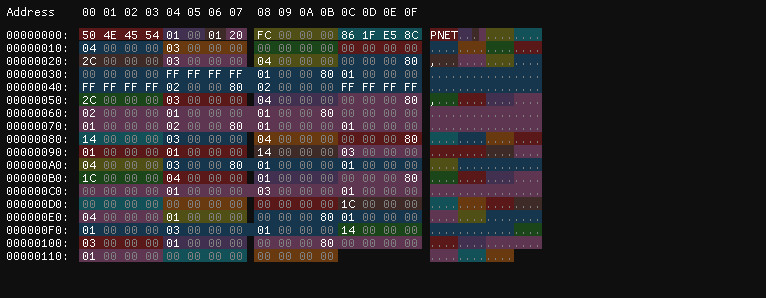
\includegraphics[width=16cm]{images/hexfile.png}
	\label{fig:hexfile}
\end{figure}

\pagebreak

\section{Algoritmo de compilação para lista de instrução}

A compilação para lista de instrução foi baseada no método de compilação para \textit{Ladder} apresentado no trabalho Petrilab \cite{de2015petrilab}, porém aqui, para lista de instrução. Fato que é possível devido à característica de que programação \textit{Ladder} pode ser gerada a partir de uma lista de instrução e vice-versa.   

Como está sendo implementando um compilador para lista de instrução, sabe-se que funcionalidades de borda de eventos e temporizadores são de fácil acesso, dispensando-se a criação de estruturas adicionais para implementação dos mesmos, e portanto, podemos compilar a rede de petri de forma mais simples, mapeando estas funcionalidades diretamente conforme necessário. Diferente da biblioteca C, onde foi desenvolvido o funcionamentos dessas funcionalidades.

Para a compilação serão definidas as seções assim como implementados na biblioteca em C.

\begin{itemize}
	\item Marcação inicial
	\item Sensibilização
	\item Disparo
	\item Lógica de saída
\end{itemize}

Cada passo será desenvolvido de forma sequencial, para ter-se esta ordem de execução de código no PLC dado.

Para compilação para código C usaremos uma função facilitadora, \lstinline{string_cat_fmt}, que é uma função feita com base na biblioteca C padrão, parecida com a função \lstinline{printf} mas que recebe uma string de formatação, a expande e concatena o resultado em um buffer de saída. Assim temos ao início um buffer vazio, e vamos inserindo as instruções até que ao final tenhamos o programa compilado. 

Também iremos utilizar as constantes \lstinline{INITIAL_RE}, que se refere a memória \lstinline{M8002} que é ativa por apenas um ciclo quando o PLC é inicializado, e \lstinline{ALWAYS}, a memória especial \lstinline{M8000}, que é sempre ativa durante a execução do código.

Como parte do algoritmo de compilação devemos definir algumas memórias temporárias e memórias para o estado da rede. Será definido que as transições e sua sensibilização via temporizador e entradas serão feitas e então armazenadas em uma memória simples, no PLC, uma memória \lstinline{M}. Transições temporizadas utilizaram uma memória auxiliar extra. Para os lugares necessitamos armazenar a quantidade de fichas atual para cada um, então utilizaremos uma unidade de memória não binária, uma memória \lstinline{word} de 16 bits, no PLC, memória tipo \lstinline{D}. As entradas e saídas serão respectivamente \lstinline{X} e \lstinline{Y}.

Ainda iremos ter um pulo condicional usado para satisfazer a condição definida na seção \ref{section:limitations}, dado no PLC pela instrução \lstinline{J}, para marcação, e \lstinline{CJ} para o pulo condicional.

Também iremos considerar a posição inicial das memórias, também as entradas, saídas e o índice do pulo condicional. Todas essas variáveis internas necessitam de um índice numérico e, portanto, o algoritmo de compilação deverá ser ciente do índice inicial para cada uma delas, para que o possa incrementar conforme a quantidade de transições, lugares, entradas e saídas. 

Temos assim a seguinte chamada de função para realização da compilação da rede de petri para lista de instrução. Percebe-se que para compilação, basta que tenhamos as informações da rede de petri e das posições iniciais.

\lstinputlisting[
	language=C,
	caption={Definição da função de compilação para lista de instrução},
	sourcePrefix={Fonte: },
	source={Do autor.},
	firstline=23,
	lastline=23,
	label=code:tpw1
]{code/tpw.c}

Dada uma rede de petri exemplo, figura \ref{fig:pnetcomp}, vamos analisar o processo de compilação, mostrando a implementação das diferentes seções, a lista de instrução para cada componente e a implementação em código C. A rede apresenta todas as funcionalidades propostas, exceto pelo arco de \textit{reset}, e demonstra uma implementação simples de um processo de exclusão mútua utilizando arcos negados, redundante, pois há apenas uma ficha em cada lugar por vez, mas demonstra um processo lógico simples. 

\begin{figure}[ht]
	\centering
	\caption{Rede de petri exemplo}
	%\incsvg{path/}{path/file}
	\incsvg{images}{images/pnetcomp}\\
	\label{fig:pnetcomp}
\end{figure}

Na rede de petri, abaixo das transições temos o evento de borda relacionado a entrada, abaixo dos lugares temos a legenda da saída e a condição lógica de ativação da mesma.

Em lista de instrução, começaremos a compilação pela marcação inicial, onde é utilizada a memória especial \lstinline{M8001} e a instrução \lstinline{MOV} para mover as fichas para os lugares iniciais, que são no PLC memórias do tipo \textit{word}.

A compilação é feita basicamente pela varredura da matriz de marcação inicial, ou seja, um laço de repetição que irá iterar pelos lugares. Assim também será realizada a implementação para os arcos, entradas e saídas, sempre utilizando as matrizes de definição, os mapas, para que possamos traduzir em código de lista de instrução.

\lstinputlisting[
	language=C,
	caption={Exemplo de lista de instrução - Marcação inicial},
	sourcePrefix={Fonte: },
	source={Do autor.},
	firstline=1,
	lastline=2,
	label=code:ilmem
]{code/il.txt}

Em código C isso pode ser implementado por um laço de repetição pelos lugares da rede de petri, onde para cada lugar, se há marcação, concatena-se a expressão em formato de lista de instrução no texto de saída final. 

\lstinputlisting[
	language=C,
	caption={Compilação da marcação dos lugares iniciais},
	sourcePrefix={Fonte: },
	source={Do autor.},
	firstline=29,
	lastline=33,
	label=code:tpwi
]{code/tpw.c}

A sensibilização das transições é relativamente fácil, e será dada como os eventos de entrada juntamente as condições de disparo, mapeadas para uma memória auxiliar que irá ser usada para movimentar as fichas. Para entradas normais temos:

\lstinputlisting[
	language=C,
	caption={Exemplo de lista de instrução - Sensibilização},
	sourcePrefix={Fonte: },
	source={Do autor.},
	firstline=18,
	lastline=20,
	label=code:ilsense
]{code/il.txt}

Para transições temporizadas, devemos além de ter se as condições de sensibilização e eventos de entrada, ter-se um temporizador. Na referência WEG TPW04, tal temporizador é dado em código como \lstinline{OUT T# K#}, onde \lstinline{T} é o índice do temporizador e \lstinline{K} a quantidade de tempo. Para transições com entrada, gera-se apenas um pulso para ativação do temporizador, por isso devemos utilizar uma memória auxiliar extra para garantir que após um pulso, o temporizador continue contando, utilizando um arranjo chamado de selo.

O Selo é basicamente uma memória auxiliar que é ativada juntamente a saída original, no nosso caso, o temporizador. E ainda mais, utiliza-se o estado desta memória como entrada auxiliar a entrada de pulso original utilizando a operação lógica ``ou''. O resultado é que quando o pulso de entrada ativa a saída e a memória auxiliar, esta mesma mantém as saídas acionadas, mesmo sem o pulso de entrada.

Para desativar o selo devemos adicionar utilizar a operação lógica ``e'' negada com as entradas e uma memória externa, que enquanto estiver em estado desligada, permitirá que a entrada acione as saídas e o selo aconteça, porém quando acionada, negará o valor das entradas, inclusive da memória selo, desativando o selo e também o temporizador. Como estamos interessados em um pulso desse temporizador para indicar sensibilização da transição, será utilizado a memória \lstinline{T} do próprio temporizador, que se torna ativa quando o mesmo termina a contagem.

Ainda mais, a memória \lstinline{T} será utilizada para com uma memória \lstinline{M}, análoga a memória auxiliar de uma transição normal, para indicar que a transição temporizada encontra-se agora sensibilizada. Assim temos o efeito geral de, quando ocorrer um pulso de entrada e as condições de disparo forem verdadeiras, um selo acontece, habilitando a contagem do temporizador que após chegar ao final da contagem irá, romper o selo, se auto desligando, e acionando com um pulso a memória auxiliar da transição.

\lstinputlisting[
	language=C,
	caption={Exemplo de lista de instrução - Sensibilização com temporizador},
	sourcePrefix={Fonte: },
	source={Do autor.},
	firstline=8,
	lastline=15,
	label=code:iltimer
]{code/il.txt}

% No disparo de transições temporizadas temos que a entrada aciona o temporizador, que quando for acionado, irá ao mesmo tempo, acionar a memória de sensibilização, irá se autorreinicializar e fará o pulo condicional para os disparos. Como visto no código \ref{code:iltimer}.

Nota-se que, para a memória auxiliar do selo, será utilizada a mesma região de memória das memórias auxiliares das transições, porém deslocada $n$ transições acima do deslocamento dado ao compilador. Assim, para uma rede de seis transições, se a segunda transição for temporizada, e o deslocamento inicial das memórias for de trinta, então temos que as memórias das transições serão \lstinline{M30, M31, M32} e a memória auxiliar de selo da terceira transição será \lstinline{M37}, dado à soma de deslocamento mais quantidade de transições mais índice da transição, $30 + 6 + 1 = 37$.

A compilação das entradas, condições e timers pode ser dada por um laço de repetição pelas transições e entradas. Caso não houverem entradas, a transição sempre dispara, e caso houverem, verifica-se se são temporizadas ou não. Caso não sejam temporizadas, implementamos o código de lista de instrução como no código \ref{code:ilsense}, caso sejam temporizadas, como no código \ref{code:iltimer}. Varremos assim, as matrizes de temporização e de entrada e verificamos se para dada transição a entrada e temporização correspondente, se houver. Em código C temos: 

\lstinputlisting[
	language=C,
	% caption={Compilação da sensibilização das entradas},
	caption={Verificação de evento de entrada e de temprização para uma transição},
	sourcePrefix={Fonte: },
	source={Do autor.},
	firstline=39,
	lastline=72,
	label=code:tpwi
]{code/tpw.c}

Note que na linha 17 em diante, com base no evento de entrada, já pode-se inserir a condição de entrada no código compilado.

Com as informações da transição, pode-se então compilar o código para mesma.

\lstinputlisting[
	language=C,
	caption={Compilação da sensibilização da transição},
	sourcePrefix={Fonte: },
	source={Do autor.},
	firstline=74,
	lastline=102,
	label=code:tpwi
]{code/tpw.c}

Como a entrada já foi inserida, basta apenas inserir as condições dos arcos, arcos de peso negativo com a instrução \lstinline{AND>=} e os arcos negados com a instrução \lstinline{AND=}, linhas 6 à 20 do código acima. E também a saída da sensibilização da transição, linha 29.

Nota-se nas linhas 2 e 23, o tratamento especial caso houver temporização para a transição, onde irá ser adicionado o código relevante a temporização, conforme o exemplo do código \ref{code:iltimer}.

Para o disparo e movimentação das fichas, deve-se adicionar as instruções de aritméticas conforme o tipo de arco. Arcos de peso negativos e positivos, que irão usar as instruções de subtração e adição para movimentação das fichas, \lstinline{SUB} e \lstinline{ADD} respectivamente, e o arco de \textit{reset}, que usa a instrução de movimentação \lstinline{MOV} com constante zero.

Para cada transição, se carrega o valor de sensibilização da mesma, e adicionam-se as instrução de movimentação. Caso hajam várias, utiliza-se a instrução \lstinline{MPS} e relacionadas para se ativar as diversas saídas. Agora para cada lugar, adicionam-se as instruções de \lstinline{ADD} para os arcos positivos, \lstinline{SUB} para os arcos negativos e de \lstinline{MOV} para os arcos de reset. Entre cada instrução devemos ler o valor da sensibilização da transição usando \lstinline{MRD}. Na última instrução de movimentação usamos \lstinline{MPP} para limpar o valor da sensibilização da pilha e escrevemos a última instrução.

Como visto na seção \ref{section:limitations}, deve-se garantir o disparo de apenas uma transição, para isso irá se utilizar um pulo condicional, que irá impedir a execução de outros disparos. O pulo será para uma marcação de execução, por exemplo \lstinline{P0}, que é localizada na instrução a frente da última instrução da última movimentação, efetivamente pulando todas os disparos. A instrução para o pulo é \lstinline{CJ}.  

\lstinputlisting[
	language=C,
	caption={Exemplo de lista de instrução - Disparo das transições},
	sourcePrefix={Fonte: },
	source={Do autor.},
	firstline=67,
	lastline=75,
	label=code:ilfire
]{code/il.txt}

Em código C temos:

\lstinputlisting[
	language=C,
	caption={Compilação da movimentação das fichas},
	sourcePrefix={Fonte: },
	source={Do autor.},
	firstline=105,
	lastline=176,
	label=code:tpwi
]{code/tpw.c}

Nas linhas 8 à 37 iremos percorrer as matrizes de arcos de peso negativos, positivos e de arco de \textit{reset}, necessário pois assim saberemos a quantidade de instruções à serem inseridos para uma transição.  

Na linha 41, começamos carregando o valor de sensibilidade da transição verificado anteriormente. Na linha 43, um laço de repetição por todos os arcos computados anteriormente, verificando se há necessidade de inserção das instruções de memória \lstinline{MPS, MRD, MPP}.

Na linhas 53 verificamos o tipo do arco a ser adicionado, adicionando as movimentações das fichas, para arco de peso negativo, a instrução \lstinline{SUB}, arco positivo a instrução \lstinline{ADD} e arco de \textit{reset}, instrução \lstinline{MOV}. 

Por fim temos as saídas, as quais só utilizam a comparação entre os lugares e uma constante dada pela matriz de saída, e após a comparação, acionam a saída física.

\lstinputlisting[
	language=C,
	caption={Exemplo de lista de instrução - Saídas},
	sourcePrefix={Fonte: },
	source={Do autor.},
	firstline=76,
	lastline=78,
	label=code:ilout
]{code/il.txt}

Nota-se na linha 1 a definição da marcação para o pulo condicional, necessário para garantir o disparo único da transições. 

Implementando, faremos um laço de repetição entre os lugares e as saídas, para cada lugar, verifica-se se há uma saída atrelada, se houver, verifica-se se o lugar possui a mesma quantidade ou mais fichas do que necessárias, usando a instrução \lstinline{LD>=} para com a memória do lugar. Então, em seguida usamos a instrução \lstinline{OUT} para redirecionar o valor da comparação para a saída atrelada. 

Em código C temos:

\lstinputlisting[
	language=C,
	caption={Compilação para as codições de saída},
	sourcePrefix={Fonte: },
	source={Do autor.},
	firstline=183,
	lastline=190,
	label=code:tpwi
]{code/tpw.c}

Na linha 2 e 3, temos os laços que irão varrer os lugares e saídas, onde verificaremos a quantidade de fichas e acionaremos as saídas, na linha 4 vemos a concatenação da instrução inteira usando \lstinline{LD>=} e \lstinline{OUT}. 
% \chapter{Resultados}

Este \textit{template} contém algumas seções criadas na tentativa de facilitar seu uso. No entanto, não há um limite máximo ou mínimo de seção a ser utilizado no trabalho. Cabe a cada autor definir a quantidade que melhor atenda à sua necessidade. 

\chapter{Conclusão}

Dados os objetivos e aspirações deste projeto, pode-se afirmar que tanto a biblioteca em C quanto o algoritmo de compilação alcançaram o resultado esperado. Para biblioteca C \cite{github-pnet} pode-se listar as seguintes estatísticas de projeto:

\begin{itemize}
	\item Commits realizados: 42
 	\item Arquivos: 21
 	\item Linhas comentadas de código: 947
 	\item Linhas de código escrito: 3368
	\item Período de trabalho: Maio 2022 - Junho 2023
\end{itemize}

Dada as especificações de projeto delimitadas, a checagem e testes deixam a biblioteca C com aspecto robusto e de pronto uso. A execução e temporização funcionam com base na biblioteca padrão C e a biblioteca \lstinline{pthread}, e portanto irão trazer performance e generalidade para aplicações desktop e compatibilidade com sistemas embarcados, através da implementação genérica a base de \textit{threads}.

Tendo opção de serialização da rede de petri em um formato de arquivo robusto, com versionamento e checagem de erro, capaz também de guardar estado, trás-se a possibilidade de um opção extra a compilação, onde dispositivos podem embarcar essas redes em formato de arquivo e carregá-las em memória no momento de execução.

A própria estrutura trás um aspecto trivial para utilização da mesma, seja na utilização das entradas e saídas de forma direta, no acesso ao estado interno, no aspecto assíncrono e também na parte da compilação, onde para maioria dos casos de utilização, dois laços de repetição, um para os lugares e outro para as transições, podem ser usados para varrer toda rede de petri, como por exemplo utilizado na compilação para lista de instrução.

Trabalhos futuros podem ser feitos sobre a parte assíncrona de temporização visto que temos o objectivo de levar essa biblioteca para sistemas embarcados. A compilação condicional de um sistema assíncrono baseado em timers de \textit{hardware} traria toda precisão e acurácia que se espera do sistema embarcado, com a rede de petri nele embutida.

O algoritmo de compilação para rede de petri foi desenvolvido de maneira bastante simples, dado a estrutura da rede em mãos e o fato da lista de instrução já suportar alguns aspectos de arquitetura já de forma nativa, como eventos de borda e temporização, abrindo então portas para implementação de outras plataformas que também usam a lista de instrução, por vezes sendo extremamente similar a referência WEG TPW04 \cite{wegtpw04}. Podendo ainda também possuir conversão da lista para outras linguagens como o próprio Ladder, aumentando o alcance dessa implementação além da própria lista de instrução.

Em sumo, os objetivos foram alcançados e espera-se que este trabalho sirva como semente para outras implementações e avanços, bem como sirva para difusão da utilização de redes de petri para modelagem de sistemas a eventos discretos, em especial a automação de sistemas industriais.
%%%%%%%%%%%%%%%%%%%%%%%%%%%%%%%%%%%%%%%%%%%%%%%%%%%%%%%%%%%%%%%%%%%%%%%%%%%%%%%%%%%%%%%%%%%%%%%%
\postextual
\addtocontents{toc}{\protect\vspace{-\cftbeforechapterskip}}						% Manter esse comando para o espaçamento correto nas referências
% \citeoption{abnt-repeated-author-omit=yes}
\bibliography{ref.bib}

% \begin{apendicesenv}
\chapter{Exemplo de Apêndice}

\label{Apend:Apend1}
Textos elaborados pelo autor, a fim de completar a sua argumentação. Deve ser precedido da palavra APÊNDICE, identificada por letras maiúsculas consecutivas, travessão e pelo respectivo título. Utilizam-se letras maiúsculas dobradas quando esgotadas as letras do alfabeto.

\end{apendicesenv}
% \begin{anexosenv}

\chapter{Exemplo de Apêndice}
\label{Anex:Anex1}
São documentos não elaborados pelo autor que servem como fundamentação (mapas, leis, estatutos). Deve ser precedido da palavra ANEXO, identificada por letras maiúsculas consecutivas, travessão e pelo respectivo título. Utilizam-se letras maiúsculas dobradas quando esgotadas as letras do alfabeto.

\end{anexosenv}
%%%%%%%%%%%%%%%%%%%%%%%%%%%%%%%%%%%%%%%%%%%%%%%%%%%%%%%%%%%%%%%%%%%%%%%%%%%%%%%%%%%%%%%%%%%%%%%%

% \appendix

% \includepdf[
%     pages={1},angle=270,turn=false,noautoscale=true,fitpaper=true,frame=false,scale=0.8,
%     pagecommand={
%         \section{Lista de materiais}
%         \label{a:lista}
%     }
% ]{../calc.pdf}

%%%%%%%%%%%%%%%%%%%%%%%%%%%%%%%%%%%%%%%%%%%%%%%%%%%%%%%%%%%%%%%%%%%%%%%%%%%%%%%%%%%%%%%%%%%%%%%%
\end{document}
%%%%%%%%%%%%%%%%%%%%%%%%%%%%%%%%%%%%%%%%%%%%%%%%%%%%%%%%%%%%%%%%%%%%%%%%%%%%%%%%%%%%%%%%%%%%%%%%

% Exemplos:

% \begin{table}[!h]
%     \centering
%     \caption{Fatores de correção por circuito.}
%     \begin{tabular}{cC{2cm}C{2cm}C{2cmt}C{2cm}C{2cm}C{2cm}}
%         \hline
%         N & Potência (\si{\volt\ampere}) & Temperatura (\si{\celsius}) & Fator de correção de temperatura & Número de circuitos & Método de referência & Fator de correção de agrupamento \\
%         \hline
%         \hline
%         \openfile{../secao_projeto1.csv}
%         \tabularfromrange{1}{2}{7}{4}
%     \end{tabular}
%     \vspace{8pt}\\
%     \caption*{Fonte: Do autor.}
% \label{tab:secao_projeto1}
% \end{table}

% \begin{figure}[h!]
%     \centering
%     \caption{Gráfico de Torque e rendimento em função da velocidade de rotação do motor CC em ligação híbrida.}
%     \includegraphics[width=17cm]{imagens/2.3.eps}
% \label{fig:2.3}
% \end{figure}

% \begin{figure}[h!]
%     \centering
%     \caption{Circuito conversor proposto.}
%     \includesvg[width=14cm]{images/2.svg}
%     \label{fig:2.1}
% \end{figure}

% \begin{table}[!h]
%     \caption{Medição de grandezas para topologia de polarização como chave - Contatos do relé abertos e $R_b$ prático}
%     \centering
%     \begin{tabular}{|c|c|c|c|}
%         \hline % 
%         $R_{b}$ (\si{K\Omega}) & $i_{c}$ (\si{mA}) & $V_{ce}$ (\si{V}) & $V_{rele}$ (\si{V}) \\
%         \hline
%         \csvreader[head to column names]{exp4.3.csv}{}{ \rb & \ic   & \vce   & \vrele}
%         \\ \hline
%     \end{tabular}
% \end{table}

% \lstinputlisting[
%     language=Octave,
%     caption={"fir\_lowpass.m"},
%     label=code:fir_lowpass
% ]{../fir_lowpass.m}
